\documentclass[times, utf8, zavrsni, numeric]{fer}
\usepackage{booktabs}
\usepackage{url}
\usepackage[final]{pdfpages}
\usepackage{amsmath}
\usepackage{blindtext}
\usepackage{enumitem}
\usepackage{listings}
\usepackage[hidelinks]{hyperref}

\renewcommand{\lstlistingname}{Programski isječak}% Listing -> Algoritam
\renewcommand{\lstlistlistingname}{Popis programskih isječaka}% List of Listings -> Popis algoritama 

\definecolor{codegreen}{rgb}{0,0.6,0}
\definecolor{codegray}{rgb}{0.5,0.5,0.5}
\definecolor{codepurple}{rgb}{0.58,0,0.82}
\definecolor{backcolour}{rgb}{0.95,0.95,0.92}
\definecolor{keyword}{rgb}{0,0,0}

\lstdefinestyle{mystyle}{
	backgroundcolor=\color{backcolour},   
	commentstyle=\color{codegreen},
	keywordstyle=\bfseries\color{keyword},
	numberstyle=\tiny\color{codegray},
	stringstyle=\color{codepurple},
	basicstyle=\footnotesize,
	breakatwhitespace=false,         
	breaklines=true,                 
	captionpos=b,                    
	keepspaces=true,                 
	numbers=left,                    
	numbersep=5pt,                  
	showspaces=false,                
	showstringspaces=false,
	showtabs=false,                  
	tabsize=4,
	inputencoding=utf8,
	morekeywords={vrati, ako, inače, za\_svaku, za\_svaki, prekini\_petlju, dok, funkcija} 
}	

\lstset{style=mystyle,texcl=true}
% set font translations
%\lstset{inputencoding=utf8}
\lstset{extendedchars=true}
\lstset{
	literate=%
	{ć}{{\'c}}1
	{č}{{\v{c}}}1
	{đ}{{\dj{}}}1
	{š}{{\v{s}}}1
	{ž}{{\v{z}}}1
	{Ć}{{\'C}}1
	{Č}{{\v{C}}}1
	{Đ}{{\DJ{}}}1
	{Š}{{\v{S}}}1
	{Ž}{{\v{Z}}}1
}

\begin{document}

% TODO: Navedite broj rada.
\thesisnumber{5173}

\title{Implementacija jezgre RTS igre}

\author{Leon Luttenberger}

\maketitle

% Ispis stranice s napomenom o umetanju izvornika rada. Uklonite naredbu \izvornik ako želite izbaciti tu stranicu.
\izvornik{}

% Dodavanje zahvale ili prazne stranice. Ako ne želite dodati zahvalu, naredbu ostavite radi prazne stranice.
\zahvala{}

\tableofcontents

\chapter{Uvod}

\chapter{Pregled vrsti računalnih igara}\label{ch:games}

% TODO Objasni što je bot
% Napiši uvod u ovo

\section{Žanr RPG}

\par Kada su osobna računala postala šire dostupna, računalne igre su počele iskorištavati kompleksniji sustav kontrola koje su omogućili miš i tipkovnica u odnosno na dosadašnje igraće palice (engl. \textit{joystick}).
Žanr igara poznat pod nazivom RPG\footnote{Igre igranja uloga (engl.\textit{Role playing games})} je nastao u to vrijeme.
Dotadašnje igre su uglavnom bili portovi arkadnih igara, poput \textit{Pacmana} ili \textit{Asteroids}.
Mana kod takvih igara je što su bile dizajnirane da kratko traju kako bi igrača natjerale da često ubacuje kovanice u automat, zbog čega su se RPS igre isticale sa svojim trajanjem.

\par U RPG igrama igrač tipično kontrolira jednog lika koji krene s ničime, obavlja razne poslove za novce, trenira svoje sposobnosti i s vremenom postaje sve moćniji. 
Neovisno o detaljima specifične igre, ideja svih igara u ovom žanru je omogućiti igraču da se poistovjeti s glavnim likom i unese u svijet u kojem se glavni lik nalazi.

\par Likovi u ovakvih igrama se tipično dijele u obične neprijatelje, ''\textit{šefove}'' i pasivne \textit{NPC}\footnote{Ne-igraći likovi (engl.\textit{Non-playable characters})} jedinice.
Obični neprijatelji su najčešći tip likova.
Njihove svrha je kako bi se borili protiv igrača, te ih tipično ima u beskonačnoj količini kako bi igrač uvijek imao nešto za raditi u svijetu.
''\textit{Šefovi}'' obično predstavljaju vođe protivničkih skupina, i kompleksniji su i teži protivnici koji se pojavljuju na kraju svakog levela ili sekcije nakon što igrač porazi mnogo slabijih protivnika.
Zamišljeni su kako bi iznenadili igrača sa svojom moći i razbili monotonost igre.
\textit{NPC} definira svakog igrača koji nije pod kontrolom igrača. Međutim, termin se obično koristi za likove u igri s kojima igrač može imati interakciju osim borbe, poput stanovnika grada ili nasumičnih ljudi koje igrač sretne tijekom igre.

\par Kako bi se svijet u kojem se igra odvija činio što stvarniji, likovi u svijetu se također moraju ponašati što realnije.
Kao posljedica toga i čistog dosega ovakvih igara, one znaju imati vrlo visoke standarde za umjetnu inteligenciju.
Primjerice, ako igrač posjeti neko selo ili grad u svijetu igre, ono mora biti ispunjeno s ljudima koji imaju svoje živote, pozadinu i posao.
Dodatna doza uvjerljivosti se postigne ako \textit{NPC}-evi u tom gradu svaki dan ujutro odu na posao, na kraju radnog dana otputuju doma i po noći spavaju.
Navedena funkcionalnost lako je izvediva uporabom nedeterminističkih konačnih automata\cite{book:AIGameProgrammingWisdom}.

\section{Žanr pucačina}

\par Postoje dvije glavne vrste pucačina: pucačine iz prvog lica, poznate kao FPS\footnote{engl. \textit{First person shooter}}, i pucačine iz trećeg lica, poznate kao TPS\footnote{engl. \textit{Third person shooter}}.
U pucačinama iz prvog lica igrač svijet promatra iz perspektive lika kojeg kontrolira, odnosno kamera se nalazi tamo gdje su njegove oči.
Suprotno tome, u pucačinama iz trećeg lika kamera se nalazi iza glavnog lika što omogućava igraču da može vidjeti model svog lika.
Bez obzira na igračevu perspektivu u ovakvim igrama, njihova premisa je vrlo jasna.
Igrač kontrolira lika koji u rukama drži nekakvo vatreno oružje te se mora boriti protiv neprijatelja.

\par Igre u ovom žanru su igrale ključnu ulogu u podizanju standarda za grafičke i mrežne performanse u računalnim igrama.
Također, kako bi bitke u igri bile što zahtjevnije, bitnu ulogu igra i razvoj botova, odnosno autonomnih agenta koji znaju pronaći svoj put na mapi, tražiti neprijatelje, skupljati oružja i boriti se.
Umjetna inteligencija iza navedenih botova je obično modelirana zasebno, kako sama igra nebi direktno ovisila o specifičnoj implementacij.
To svojstvo omogućava proširivost samo igre, odnosno omogućava programerima da napišu svoje implementacije te ih testiraju u samoj igri.

\par Zahvaljujući navedenom svojstvu, neke igre u ovom žanru se često koriste u istraživanjima umjetne inteligencije.
Uvjeti u takvim igrama mogu biti puno bliži uvjetima u stvarnom svijetu nego čisti laboratorijskih uvjeta, što omogućava efektivno testiranje novih i bržih algoritama.

\section{Platformeri}

\par Platformeri su jedan od starijih žanrova računalnih igara.
One su tipično prikazane u 2D svijetu, u kojima igrač započne igru na dnu ekrana i cilj je pomoću pravovremenih skokova po platformama popesti se na vrh.
Na putu do cilja, igrač će susresti protivničke jedinice koje je cilj izbjeći.

\par Zbog ograničenosti računala u doba kada je ovaj žanr nastao, protivničke jedinice su strogo skriptirane, npr.\ beskonačno se kreću lijevo-desno po svojoj platformi.
Kao posljedica toga, igranje ovakvih igra se pretežno svodi na predviđanje idućih događaja u igri.

\section{Trkaće igre}
% Nekoliko rečenica o ovome


\section{Sportske igre}
% Nekoliko rečenica i o ovome

\chapter{RTS igre}\label{ch:rtsGames}

\par RTS žanr računalnih igara temelje se na skupljanju resursa za izgradnju jedinica i građevina s ciljem da se poraze protivnici. 
Za razliku od strategija na potez (engl. Turn-based strategy) gdje svaki igrač ima proizvoljno vrijeme za odigrati svoj potez, u RTS igrama svi igrači igraju svoje poteze u isto vrijeme znajući da svi protivnici rade isto. 
U širem smislu, RTS igra se može definirati kao simulacija bitke u stvarnom vremenu.

%TODO napisi o cemu ce sve bit poglavlje

\section{Elementi RTS žanra}

\par Tipična RTS igra sastoji se od mnogih različitih elemenata.
Prije svega, svaka igra se odvija na mapi ograničene veličine koja je određena s raznim tipovima terena, poput trave, vode, planina, pustinje, itd. 
Tip terena može odrediti koje se jedinice mogu kretati po njemu.
Primjerice, pravila igre mogu biti takva da se običan vojnik ne može kretati po vodi, dok neki drugi tip jedinice poput broda može.
Kao posljedica toga, teren igra veliku ulogu jer može zahtijevati korištenje posebnih strategija.

\par Još jedna bitan element RTS igara je skupljanje resursa.
Ovisno o konkretnoj igri, resursi mogu biti drvo, minerali, nafta, zlato, itd. Oni se tipično skupljaju s posebnom vrstom jedinica zvanom radnicima, te se koriste za izgradnju novih jedinica, zgrada, radnika, itd.
Resursi također igraju veliku ulogu u strategiji same igre.
Primjerice, ako se igrač nalazi u situaciji gdje ne može dalje napredovati zbog manjka nekog resursa, bit će prisiljen otići u potragu za istim.
Analogno tome, višak izvora nekog resursa igrača može postaviti u opasnost jer će ostalim sudionicima igre biti prioritet napasti s ciljem da se ukradu resursi.

\par Osim resursa i mape, bitan element u svakoj RTS igri je izgradnja zgrada. 
Konkretne igre obično imaju mnogo različitih zgrada od kojih svaka ima svoj skup funkcionalnosti, poput treniranja novih jedinica, procesiranje resursa, istraživanje novih tehnologija, itd.  

\par Posljednji bitni element igara u RTS žanru su jedinice. 
Svaka igra ima skup različitih jedinica koje igrač može odabrati i izgraditi za svoju vojsku.
Svaka vrsta jedinice može imati svoje prednosti i mane.
Npr.\ igra može kao vrstu jedinice imati konjanika koja ima prednost brzog kretanja po mapi, no ima manu da je izrazito ranjiv na kopljanike.

\par Jedna od posebnosti žanra RTS je činjenica da svi dosad navedeni elementi nisu direktno ovisni jedni o drugima.
Mapa može biti definirana izvan same igre u nekom vanjskom uređivaču mapa, dok jedinice, resursi i zgrade ne moraju ništa konkretno znati jedni o drugima.
Jedinice će samo znati da se kreću po terenu čiji koji ima neke definirane karakteristike, te će samo znati da napada protivničke zgrade i jedinice. 
Zgrade i resursi mogu biti definirani samo kao objekti na mapi, gdje će bilo kakva daljnja funkcionalnost ovisiti o konkretnoj igri.

\par Takva struktura može omogućiti da se određene komponente iz igre višestruko iskorištavaju te da se nove funkcionalnosti mogu lakše dodavati u igru.
Primjer ovakve strukture implementiran je u okviru ovoga rada, te su detalji više obrađeni u poglavlju~\ref{ch:implementation}.

\section{Strategija}

\par Glavni cilj u igrama u RTS žanru analogan je igrama poput šaha, odnosno cilj je pametnom uporabom vlastite vojske poraziti vojsku od suparnika. 
Za razliku od šaha, u računalnim strateškim igrama igrač započne igru \textit{praznih ruku}, odnosno igru može započeti sa samo jednim radnikom čiji je posao skupiti prve resurse s kojima će izgraditi prve jedinice te nove radnike i zgrade.

\par Igrač jedinicama daje naredbe tako da ih odabere (npr.\ pritiskom tipke miša) i zada im odredište gdje se moraju pomaknut ili protivničku jedinicu koju moraju napasti. 
Igrač također može odabrati zgradu i njoj dati naredbu što da proizvodi, poput novih jedinica ili istraživanja novih tehnologija koje će omogućiti izgradnju novih tipova jedinica i zgrada.

\par Odluke u RTS igrama mogu se podijeliti u dvije kategorije: mikro upravljanje i makro upravljanje. 
Makro upravljanje predstavlja odluke na višoj razini apstrakcije poput odluka koje zgrade i jedinice graditi, kada krenuti u napad, itd. 
Mikro upravljanje svodi se na upravljanje pojedinim jedinicama.
Dobro taktičko pozicioniranje jedinica i fokus na najjače protivničke jedinice u dosegu često mogu definirati ishod igre.\cite{article:HybridPathdinding}

\par Kao posljedica svega navedenog, evidentno je da je strategija centralnih aspekt igara u RTS žanru. 

\par Također, bitno je naglasiti da će određene strategije funkcionirati samo protiv pojedinih protivnika i da određene situacije mogu zahtijevati promjenu strategije. 
Primjerice, igrač se može odlučiti za strategiju ranog napada (engl. \textit{rush strategy}), odnosno odmah se fokusirati na izgradnju velikog broja osnovnih borbenih jedinica koje će što ranije moguće poslati u napad na protivnika.
Kao kontrast tome, protivnik se može fokusirati na razvoj tehnologije što će ga ostaviti ranjivim na početku igre, ali će mu u kasnijim fazama igre omogućiti da gradi jedinice koje su jače od protivničkih.

\section{Izazov za umjetnu inteligenciju}

\par RTS igre predstavljaju razne izazove za razvoj umjetne inteligencije. 
Iz perspektive mikro upravljanja, umjetna inteligencija mora imati sustav po kojem će određivati najkraći put do odredišta, te kako se treba ponašati u slučaju da na putu naiđe na nešto ne planirano, poput protivničkih jedinica ili promjena na terenu. 
S druge strane, makroupravljanje je mnogo složeniji izazov za umjetnu inteligenciju jer se sustav mora odrediti dugotrajne ciljeve, npr.\ hoće li se fokusirati na jaku vojsku, tehnološki ili ekonomski razvoj, itd.

\par Navigacija jedinica je u RTS igrama često najintenzivniji posao za računalni procesor.
Veliki broj jedinica stvara potrebu za velikim brojem pretraga, pogotovo ako se svaka kreće u svom smjeru, te svaka od njih mora pratiti potencijalne promjene na terenu i promijeniti ponašanje u skladu s istima.
Tehnike poput skupljanja jedinica u grupe kako bi se zajedno kretali prema cilju mogu smanjiti taj trošak, jer će se sve pretrage i provjere izvršavati nad tom grupom jedinica\cite{book:AIGameProgrammingWisdom}. 

\par Na slici~\ref{fig:RTSgrouping} prikazane su tri jedinice kako se zajedno kreću prema bijeloj linij koja označava najkraću putanju.
Pretraga je obavljena za čitavu grupu odjednom, umjesta za sve jedinice zasebno, što je značajno smanjilo trošak izračuna puta.

\begin{figure}[h] 
	\centering
	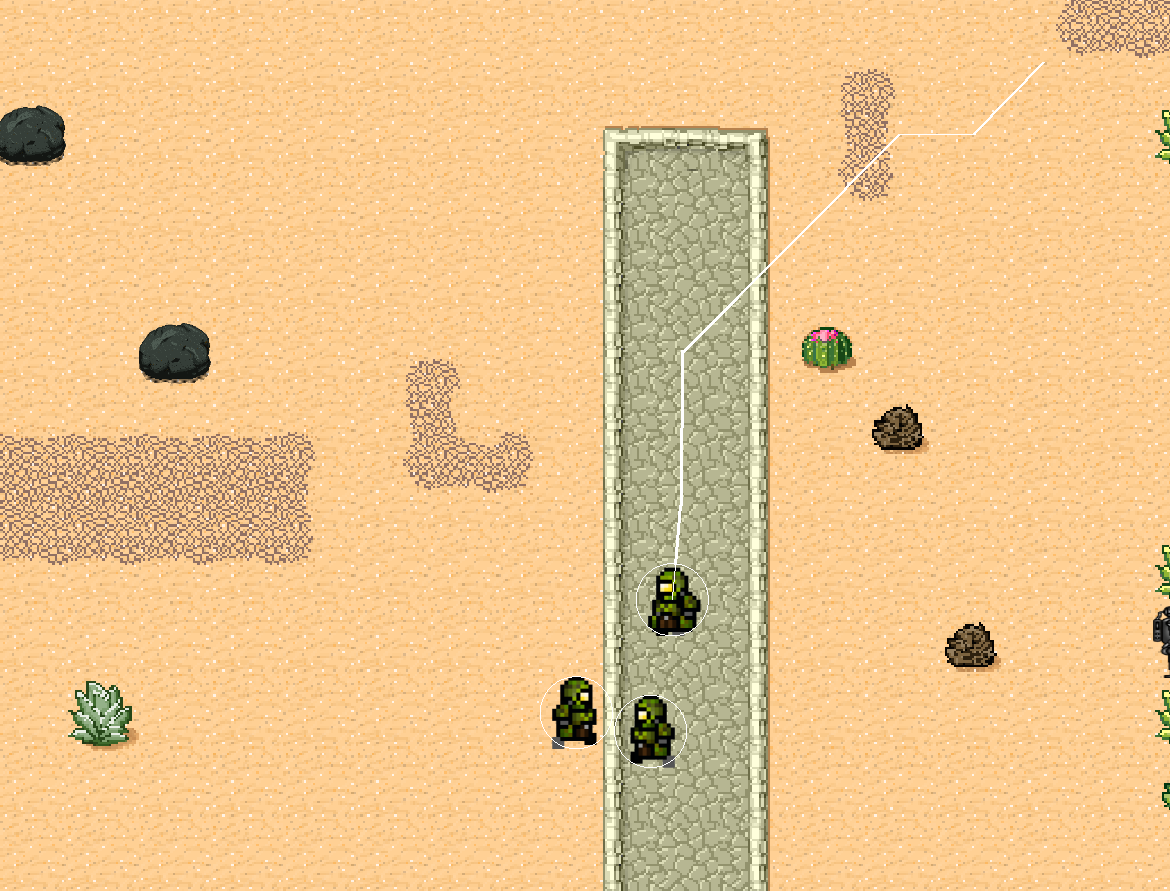
\includegraphics[width=0.6\linewidth]{images/RTSgrouping.png}
	\caption{Zajedničko kretanje jedinica}
	\label{fig:RTSgrouping}
\end{figure} 

\par Jedinice se također moraju znati ponašati u borbi na što pametniji način. Primjerice, strijelac bi se trebao držati na udaljenosti od mete jer je tamo najopasniji.
U trenutku kada se nađe u borbi prsa u prsa, njegova najbolja strategija je povući se na udaljenost iz koje može pucati.
Međutim, osposobiti i igračeve jedinice da se ponašaju na navedeni način  je dvosjekli mač.
S jedne strane, jedinice će biti sposobnije i igrač neće morati konstantno mikro-upravljati njima.
Međutim, navedenu prednost će neki igrači smatrati manom.
Ako su strijelci dovoljno pametni da se znaju držati na udaljenosti iz koje mogu pucati i povlače se kada dođu u opasnost, to eliminira potrebu za nekim strategijama s kojima su dugogodišnji igrači strategija dobro upoznati.
Primjer takve strategije je napraviti formaciju strijelaca tako da budu u jednoj liniji, te između njih i neprijatelja postaviti mačevalce koji će sprječavati protivnike da se približe.

% Možda ubaci sliku

\par Umjetna inteligencija koja će upravljali strategijom na višoj razini slična je ulozi generala u vojsci. 
Ona dobiva percepcije o trenutnom stanju na terenu od njenih jedinica.
Na temelju tih percepcija računalo može bitno promijeniti trenutnu strategiju. Primjerice, ako je računalo negdje otkrilo izvore resursa, ono može napraviti odluku da radnike pošalje u tom smjeru kako bi skupili što više toga.
Nadalje, ako se taj resurs može koristiti za razvoj tehnologije, u trenutku kada ga se skupi dovoljno računalo može promijeniti dugotrajni cilj u igri na tehnološki razvoj.

\par Dugotrajni ciljevi mogu ovisiti i o tome s kojom se frakcijom igra. 
Npr.\ jedna frakcija će preferirati izgradnju što veće vojske dok će druga raditi sve što može kako bi razvila stabilnu ekonomiju.
Navedene karakteristike mogu pojedinim frakcijama dati različite osobnosti.
Kada se to iskombinira sa specifičnim tipovima jedinica za pojedine frakcije, postigne se velika razlika između svih računalnih protivnika na razini njihove umjetne inteligencije.

\par Još jedan izazov za makro-strategiju je izgradnja građevina.
One se moraju postaviti u relativnoj blizini kako bi se lakše mogle štititi.
Zgrade koje obrađuju resurse bi trebale biti u blizini resursa koji se obrađuje, defenzivne zgrade trebaju biti na mjestima gdje će pružati maksimalnu zaštitu, poput u prolazima iz kojih se neprijatelji najčešće približavaju.

\section{Primjeri popularnih RTS igara}

\subsubsection{Starcraft}
\par \textit{Starcraft} je vojna RTS igra koju je izdao \textit{Blizzard Entertainment} 1998.\ godine. 
Smatra se jednom od najbitnijih i najutjecanijih igara svim vremena te je jedna od igara koja je definirala RTS žanr.

\par Radnja je smještena u 25.\ stoljeću i vrti se oko tri frakcije koje se bore za dominaciju u dalekom dijelu Mliječne galaksije. 
Svaka frakcija ima vlastite prednosti i sposobnosti po kojima se razlikuje od ostalih. 
Frakcija \textit{Protoss}, koju čini rasa humanoidnih tehnološki naprednih vanzemaljaca i psihičkim moćima, ima pristup jakim jedinicama i naprednim tehnologijama.
Međutim, budući da je razvoj njihovih jedinica skup i dugotrajan proces, igrači su potaknuti da slijede strategiju kvalitete umjesto kvantitete.
Frakcija \textit{Zerg}, koju čini rasa insektoidnih vanzemaljaca u potrazi za genetskim savršenstvom i opsjednuti sa asimilacijom ostalih rasa, posjeduje samo organske jedinice i strukture koje se mogu proizvesti brzo i jeftino.
Zadnja frakcija su \textit{Terrani}, odnosno ljudi progonjeni sa Zemlje.
Oni predstavljaju sredinu između prijašne dvije rase, odnosno jedinice su im fleksibilne i sposobne za mnogo različitih poslova.

\par Dokaz uspiješnosti \textit{Starcrafta} je činjenica da se nakon 20 godina i dalje aktivno igra.
Igra je također imala dovoljno veliki utjecaj da ostvari status profesionalnog sporta u Južnoj Koreji.

\subsubsection{Age of Empires}

\par \textit{Age of Empires} serijal RTS igara proizveo je \textit{Ensemble Studios} i izdao \textit{Microsoft Studios}. 
Istoimena prva igra u serijalu izašla je 1997.\ godine.

\par Radnja je smještena tijekom povijesti, gdje igrač mora izgraditi i unaprijediti vlastitu civilizaciju.
Prva igra odvija se od kamenog doba do željeznog doba, no kasnije igre su promjenile fokus na novija vremenska razboblja, poput srednjeg vijeka u \textit{Age of Empires II} i razdoblja kolonizacije Amerike u \textit{Age of Empires III}.
Igrač započinje igru s nekoliko seljaka s kojima mora skupljati resurse kako bi gradio nove jedinice, proširivao selo i istraživao nove tehnologije.

\par Tijekom razvoja igri u ovom serijalu, veliki naglasak je bio na razvoju umjetne inteligencije.
Cilj razvojnog tima bio je napradiviti umjetnu inteligenciju koja koristi taktike i strategije za pobjediti, umjesto da dobiva dodatne resurse i jače jedinice kako bi imala bolju šansu za pobjediti igrača, kao što igre često rade.
Dodatna sposobnost umjetne inteligencije je što se prilagođava taktikama igrača, odnosno pamti koje je igre pobjedila ili izgubila te s vremenom postaje sve bolji.

\chapter{Kretanje jedinica}\label{ch:pathfinding}

\section{Pretraživanje prostora stanja}\label{sec:stateSearch}

\par Pretraživanje prostore stanja može riješiti mnogo analitičkih problema, uključujući pronalazak najkraćeg puta. 
Ako korisnik odabere jedinicu koja se nalazi na početnoj poziciji i zada joj odredište, jedinica će pretragom prostornog stanja pronaći slijed akcija koji definira optimalni put.

\par Problem pretrage \(S\) možemo formulirati sa šestorkom
\[(S, S_0, akcije(s), prijelaz(s, a), cilj(s), cijena(s, a))\]
u kojoj su:
\begin{itemize}
    \item \(S\) skup stanja.
    \item \(S_0\) početno stanje.
    \item \(akcije(s)\) skup mogućih akcija u stanje \(s\).
    \item \(prijelaz(s, a)\) stanje dobiveno kada se izvede akcija \(a\) u stanju \(s\).
    \item \(cilj(s)\) ispituje jeli stanje \(s\) ciljno stanje.
    \item \(cijena(s, a)\) cijena akcije \(a\) kada smo u stanju \(s\). 
\end{itemize}

\subsection{Neusmjerena pretraga}

\begin{figure}[h] 
	\centering
	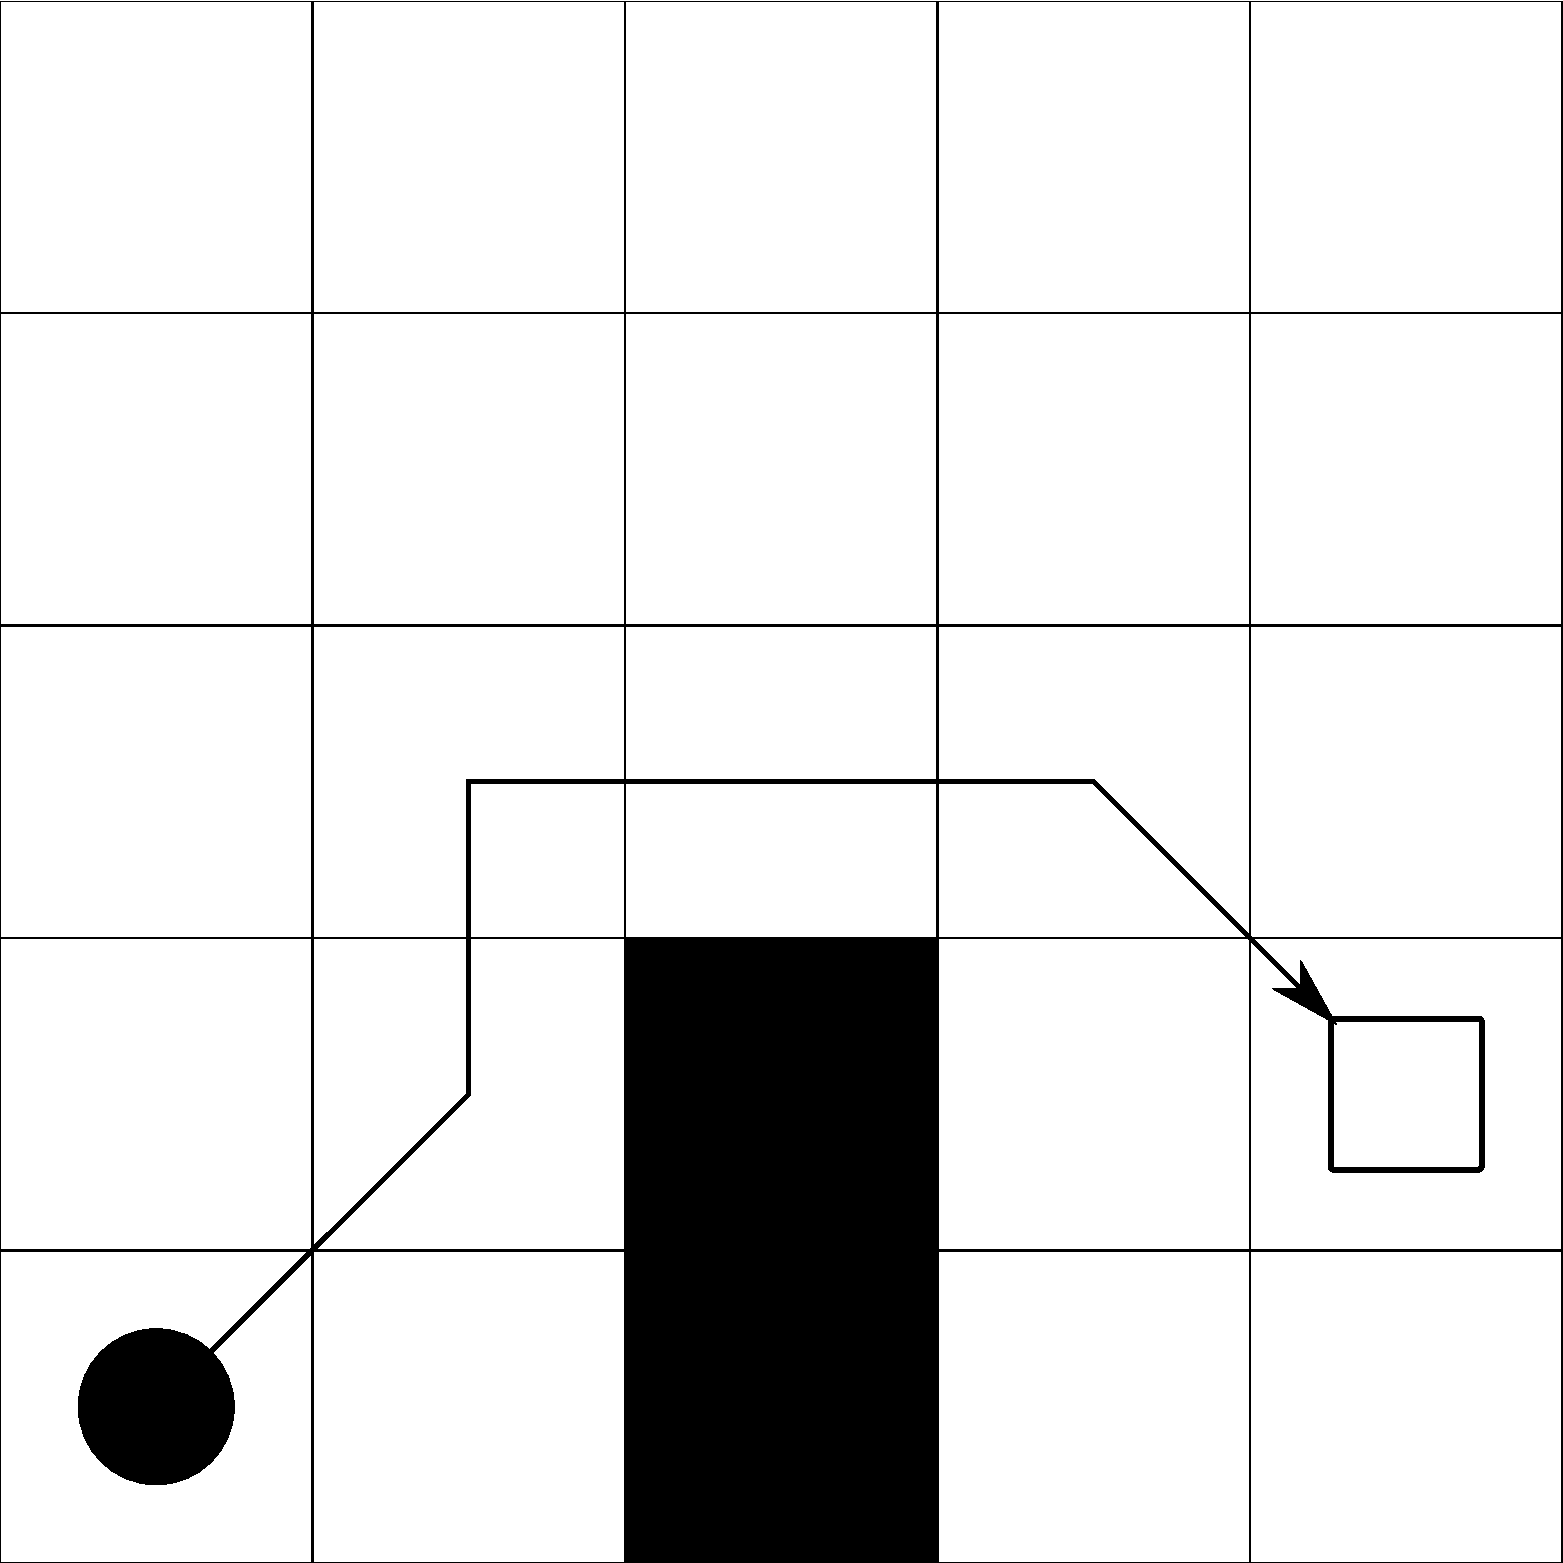
\includegraphics[width=0.3\linewidth]{images/basicGrid.pdf}
	\caption{}
	\label{fig:basicGrid}
\end{figure} 

Na slici~\ref{fig:basicGrid} prikazan je rezultat pretrage najkraćeg puta na 5x5 ploči na kojoj su mogući i dijagonalni prijelazi.
Ispunjeni krug predstavlja početnu poziciju, prazan kvadrat predstavlja cilj te ispunjeni kvadrati predstavljaju prepreke.
Ako definirano da se pločica u donjem lijevog predstavlja s koordinatama \((0, 0)\), tada standardna formulacija problema glasi:
\begin{itemize}
    \item \(S\): sve pozicije od \((0, 0)\) i \((4, 4)\).
    \item \(S_0\): stanje \((0, 0)\).
    \item \(akcije(s)\): predstavlja prijelaze s kojima se može doći do susjednih polja od \(s\) koji nisu prepreke. 
    Moguće vrijednosti su: \textit{gore}, \textit{dolje}, \textit{lijevo}, \textit{desno}, \textit{gore-lijevo}, \textit{dolje-lijevo}, \textit{gore-desno} i \textit{dolje-desno}. 
    Npr.\ za početno stanje \(S_0\) funkcija će vrati slijed: \textit{gore}, \textit{desno} i \textit{gore-desno}. 
    \item \(prijelaz(s, a)\): funkcija vraća novu poziciju na polju kada se akcija \(a\) izvrši iz stanja \(s\). Npr. \(prijelaz((0, 1), gore)\) će vratiti stanje \((1, 1)\).
    \item \(cilj(s)\): funkcija je zadovoljena samo za \((4, 1)\).
    \item \(cijena(s, a)\): cijene prijelaza su Euklidove udaljenosti, odnosno prijelazi na strogo susjedna polja imaju cijenu \(1\), dok dijagonalni prijelazi imaju trošak \(\sqrt{2}\).
\end{itemize}

\par S obzirom na činjenicu da cijene prijelaza nisu uvijek iste, najbolje je odabrati algoritam pretrage koji uzima u obzir cijenu puta.
Najosnovniji takav algoritam pretrage je \textbf{pretraživanje s jednolikom cijenom} (engl. \textit{uniform-cost search}).

\par U isječku~\ref{fig:codeUCS} prikazan je pseudokod za algoritam pretraživanja s jednolikom cijenom. 
Algoritam inicijalizira početni čvor, prioritetni red sortiran po cijeni puta \(g(s)\) i skup posjećenih stanja. 
Prioritetni red je struktura u koju ubacujemo elemente koji se mogu sortirati po zadanom kriteriju i uvijek izvlačimo najveći ili (u ovom slučaju) najmanji element.
Algoritam zatim uvijek uzima čvor s najmanjom vrijednosti i provjerava ako je stanje u tom čvoru ciljno stanje.
Ako je uvijet ispunjem, algoritam vraća to rješenje.
U protivnom, čvor se dodaje u skup posjećenih stanja i dalje se proširuje, odnosno njegovi susjedi se dodaju u prioritetni red.
Bitno je naglasiti zadnji korak u proširanju stanja, odnosno provjeri jeli čvor s istim stanjem već ubačen u prioritetni red ali s većim troškom.
U tom slučaju, potrebno je zamijeniti čvor u prioritetnom redu s novim čvorom.
Ovime osiguravamo da u trenutku kada se čvor izvuće iz prioritetnog reda, najkraći put do njegovog stanja je pronađen.

\begin{minipage}{\textwidth}
	\lstinputlisting[caption = {Pseudokod za pretraživanje s jednolikom cijenom},
    label={fig:codeUCS}]{codesnippets/ucs.txt}
\end{minipage}

\par Zbog navedenog svojstva, algoritam pretraživanja s jednolikom cijenom je \textbf{optimalan}, odnosno uvijek će pronaći optimalni put do odredišta ako ono postoji.

\par Unatoč tome što će algoritam uvijek pronaći najkraći put, ponekad će za to morati posjetiti veliki broj stanja jer se u obzir uzima samo cijena puta, bez znanja o tome dali je taj čvor bliži cilju ili ne. 
Zbog ovog svojstva pretraživanje s jednolikom cijenom čini jedno od neusmjerenih algoritama pretrage.

\subsection{Usmjerena pretraga}

\par Usmjereni algoritmi pretraživanja su algoritmi koji koriste heurističku informaciju kako bi se pretraživanje brže usmjerilo prema cilju.
U općenitom obliku ovakvog algoritma stanja se ubacuju u prioritetni red kao u pretraživanju s jednolikom cijenom, no umjesto da se koristi cijena puta \(g(s)\) koristi se \textbf{evaluacijska funkcija} \(f(s)\).

\par Odabir evaluacijske funkcije \(f\) definira strategiju pretrage. 
Funkcija \(f\) tipično ima kao komponentu \textbf{heurističku funkciju} \(h\), koja se definira kao procjena minimalnog troška puta od trenutnog čvora do cilja\cite{book:AIModernApproach}.

\par Primjer takvog pretraživanje je pohlepno pretraživanje. 
Ono odabire onaj čvor koji se čini najbliži cilju, ne uzimajući u obzir trošak puta.
Evaluacijska funkcija \(f(s)\) se definira kao \(f(s) = h(s)\).

\par Poboljšanje tog algoritma je ujedno i najpoznatija implementacija usmjerene pretrage: \textbf{algoritam A*}. 
U njemu se čvorovi evaluiraju tako da se zbroji trošak puta \(g(s)\) i heuristika \(h(s)\):
\begin{equation}
f(s) = g(s) + h(s).
\end{equation} 

Prema tome, vrijednost \(f(s)\) predstavlja procjenu troška puta koji prolazi kroz stanje \(s\).
Ovaj algoritam je identičan pretraživanju s jednolikom cijenom, osim što se u prioritetni red za čvorove ubacuje vrijednost \(g(s) + h(s)\) umjesto \(g(s)\).

\subsubsection{Uvjeti za optimalnost algoritma A*}
Kako bi algoritam A* bio optimalan, heuristika mora zadovoljiti sljedeća dva svojstva: \textbf{optimističnost} i \textbf{konzistentnost}.

\par Heuristika je optimistična ako nikad ne predvidi udaljenost do cilja koja je veća od stvarne. 
Kao posljedica činjenice da je \(g(s)\) cijena puta do stanja \(s\), \(f(s)\) nikad neće imati vrijednost veću od cijene stvarnog puta do cilja kroz čvor \(s\).
Matematički formulirano, ako je \(h^*(s)\) cijena stvarnog puta od čvora \(s\) do cilja, tada vrijedi:
\begin{equation}
\forall s \in S, h(s) \leq h^*(s).
\end{equation} 
Također, vrijednost heuristike u ciljnom čvoru mora biti 0: \(h(s_{cilj}) = 0\).

\par Heuristika je konzistentna ako procjena udaljenosti do cilja nikad nije veća  od zbroja heurističke vrijednosti od susjednog stanja i cijeni puta između navedena dva stanja.
Odnosno, ako je \(s\) trenutno stanje, \(s'\) susjedno stanje i \(a\) akcija koja vodi iz \(s\) u \(s'\), tada vrijedi:
\begin{equation}
h(s) \leq c(s, a) + h(s').
\end{equation} 
Ovo svojstvo je temeljeno na principu nejednakosti trokuta, odnosno činjenici da zbroj duljina dviju stranica trokuta ne može biti manja od duljine treće stranice, što se može uočiti na slici~\ref{fig:triangleInequality}.

\begin{figure}[h]
	\centering
	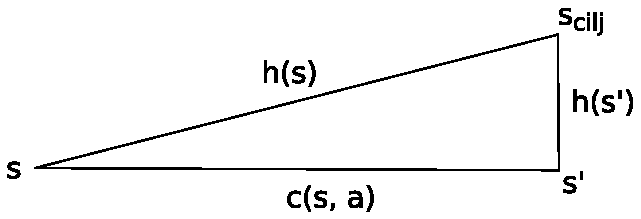
\includegraphics[width=0.5\linewidth]{images/triangleInequality.pdf}
	\caption{Veza između konzistentnosti heuristike i nejednakosti trokuta}
	\label{fig:triangleInequality}
\end{figure} 

\par Konzistentna heuristika je ujedno i optimistična, iako suprotno ne vrijedi. 
Samim time, konzistentnost je stroži uvjet od optimističnosti. 
U algoritmu A* konzistentnost heuristike osigurava da će se čvor proširiti kada je najkraći put do njega pronađen, poput pretraživanja s jednolikom cijenom.

\par Još jedno bitno svojstvo heuristike je \textbf{obaviještenost}. 
Jedan primjer heuristike koja zadovoljava uvjet optimističnosti i konzistentnosti je funkcija koja za svako stanje vraća 0: \(\forall S \in S, h(s) = 0\). 
Algoritam A* s ovakvom heuristikom degenerira pretraživanje s jednolikom cijenom, odnosno za svako stanje se gleda samo njegova cijena \(g\). 
Heuristika je bolja ako daje više informacija, odnosno ako funkcija \(h\) vraća veću vrijednost.

\section{Prilagodba na promjene}\label{sec:adaptation}

\par Likovi u računalnim igrama se moraju kretati glatko bez nepotrebnih stajanja, što znači da moraju pretraživati u realnom vremenu.
Nakon što se pretraga izvršti, agent\footnote{objekt koji je izvršio pretragu} se mora fizički pomaknuti prema cilju.
U međuvremenu se na mapi mogu dogoditi razne promjene na koje se agent mora znati prilagoditi.

\par A* sam po sebi nije prikladan za taj posao, jer broj stanja koji se moraju pretražiti raste ovisno o ukupnom broju stanja. 
Također, A* ne zna prepoznati promjene u prostoru stanja, poput promjena na mapi. Kada bi se prilikom dolaska u svako novo stanje algoritam A* ponovo izvrtio, u najboljem slučaju jedinice bi u svakom novom stanju zastale dok se prostor pretraži te im kretanje ne bi više bilo glatko. 
U najgorem slučaju, čitava igre bi bila sklona čestim zaustavljanjima (engl. \textit{lag spike}).

\subsection{Ponovljeni A*}

\par Najjednostavnija modifikacija koja se može napraviti nad algoritmom A* kako bi bio iskoristiv u realnom vremenu je ograničenje pretrage na manji lokalni prostor kojeg agent može dostignuti u određenom broju poteza. 
Konkretno, postavi se ograničenje na broj stanja koji se mogu pretražiti i ograničenje na broj poteza koje agent može napraviti.
Kada se pretraga iz trenutne pozicije izvrši, agent će krenuti prema stanju koje je trenutno sljedeće u prioritetnom redu sve dok ga ne dosegne ili dok ne napravi maksimalni broj dozvoljenih poteza.
Taj će se postupak ponavljati sve dok agent ne dođe do ciljnog položaja.
Dodatno, može se definirati uvjet da ako se promjeni stanje koje se trenutno nalazi u trajektoriji (npr.\ ako se direktno na putu jedinici u RTS igri izgradi zgrada), pretraga se ponovi s novim podatcima o okolini.

\par Zahvaljujući navedenim modifikacijama, algoritam A* se može koristiti u stvarnom vremenu. 
Broj posjećenih stanja bit će neovisan broju mogućih stanja što garantira mali prostor stanja, no rezultirat će dužim putevima agenta do cilja.

\begin{figure}[h]
	\centering
	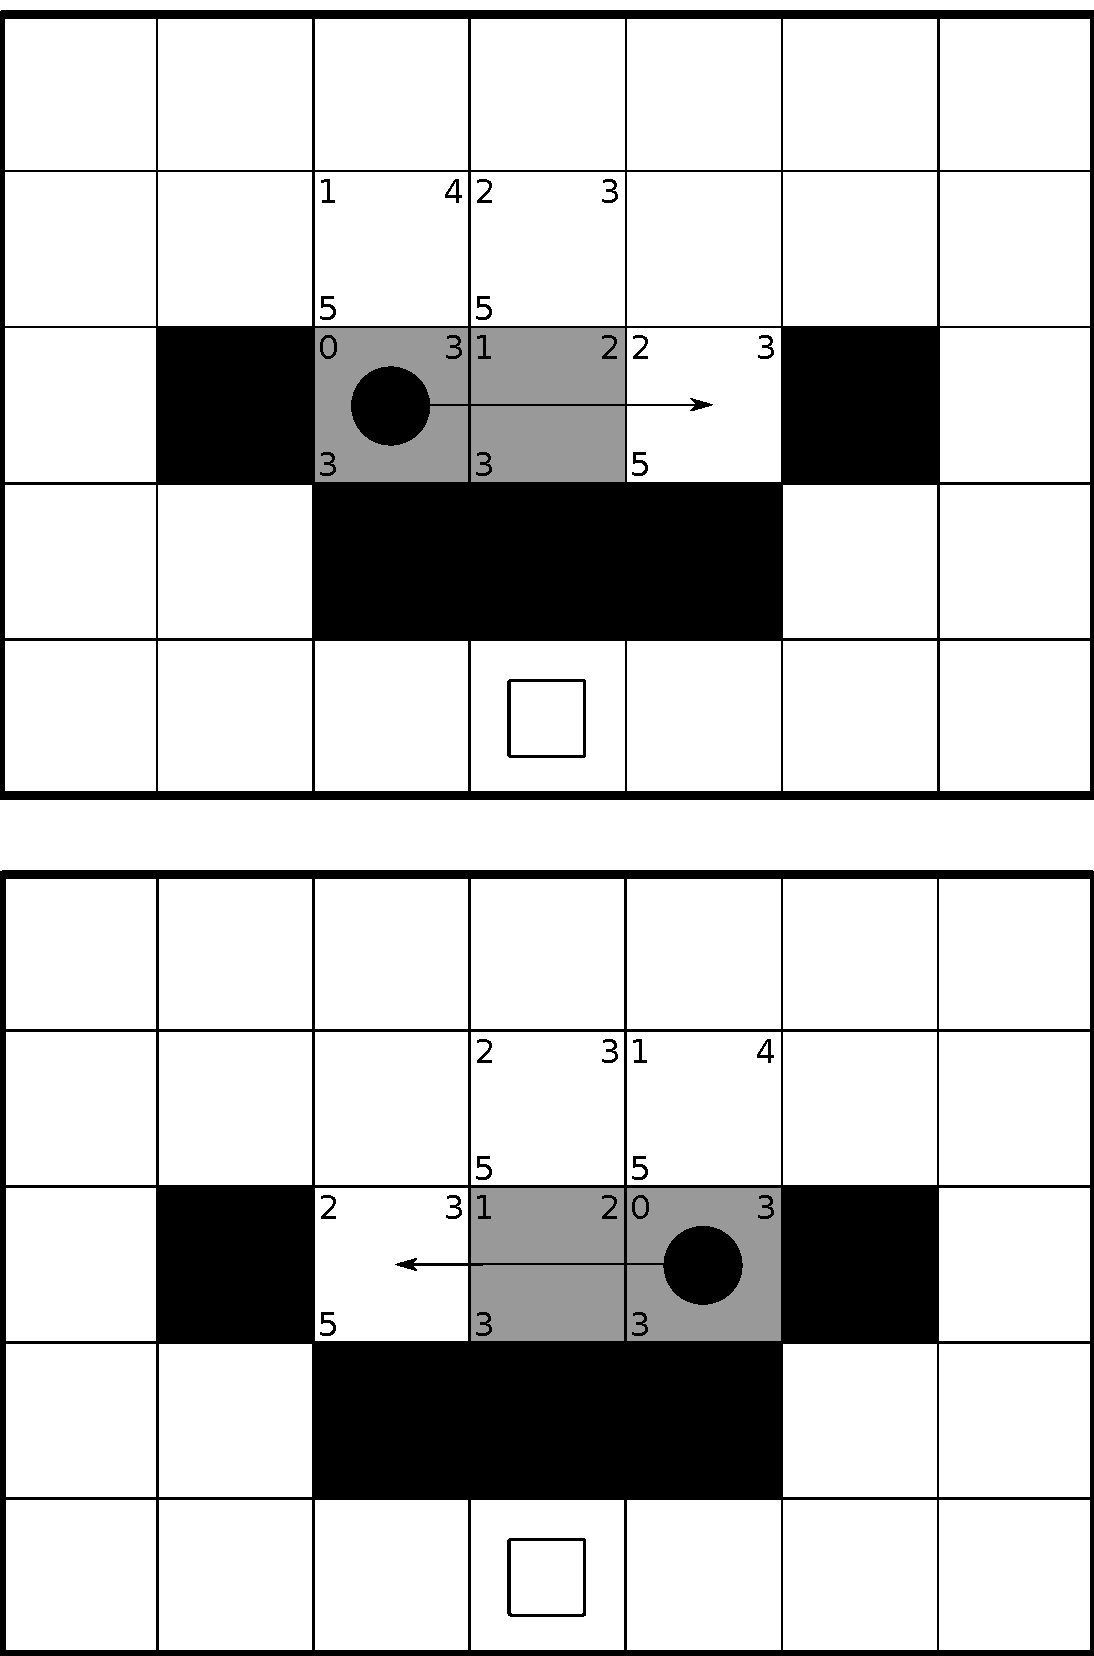
\includegraphics[width=0.45\linewidth]{images/repeatedAStarCycle.pdf}
	\caption{Pojava ciklusa kod ponovljene pretrage}
	\label{fig:pathfindingCycle}
\end{figure} 

\par S obzirom na činjenicu da svaka pretraga kreće ispočetka, moguća je pojava ciklusa. 

\par Na slici~\ref{fig:pathfindingCycle} prikazan je rezultat pretrage koja je rezultirala ciklusom. 
Radi jednostavnosti, u ovom problemu dopušteni su samo pomaci na izravno susjedna polja.
Broj stanja koja se mogu pretražiti ograničen na 2, te je agent zatim otišao prema idućem čvoru u prioritetom redu. 
Ispunjeni krug predstavlja početni položaj u pretrazi, kvadrat ciljni položaj, dok zasivljeno polje predstavlja pregledano stanje. 
U gornjem lijevom kutu zapisan je trošak puta za čvor \(g(n)\), u gornjem desnom kutu vrijednost heuristike \(h(n)\) te u donjem lijevom kutu vrijednost \(f(n) = g(n) + h(n)\).
U slučaju kada se u prioritetni red doda čvor s vrijednosti koja već postoji, prvi u redu je onaj koji je zadnji dodan.

\subsection{Adaptivni A* u stvarnom vremenu}
\par Kako bi se riješio problem pojave ciklusa, potrebno je sačuvati informacije iz prijašnjih pretraga.
Jedan od algoritama koji nudi takvu mogućnost je adaptivni A* u stvarnom vremenu (engl. \textit{Real-Time Adaptive A*}, u nastavu RTAA*).

\par Neka je potrebno izvesti više A* pretraga s konzistentnom heuristikom i istim ciljnim stanjem no s različitim početnim stanjima. Adaptivni algoritam A* će nakon svake pretrage podesiti heurističke vrijednosti posjećenih stanja kako bi buduće pretrage bile obavještenije\cite{article:RTAAStar}.

\par Neka je \(s_{start}\) početno stanje u pretrazi i \(s\) stanje u lokalnom prostoru stanja. Ako je heuristika \(h\) konzistentna vrijedi relacija:
\begin{equation}
\forall s \in S, h(s_{start}) \leq g(s) + h(s).
\end{equation}
Drugim riječima, put od početne pozicije do cilja kroz stanje \(s\) nikad neće biti veće od stvarne udaljenosti od početnog stanja do cilja.

\par Ako je stanje \(\overline{s}\) prvo stanje u prioritetnom redu kada je lokalna pretraga završila, uvrštavanjem uvjeta konzistentnosti u gore navedenu formulu dobiva se sljedeći izračun:
\begin{equation}
\begin{aligned}
& \forall s \in S, f(\overline{s}) \leq g(s) + h(s)\\
& \forall s \in S, h(s) \geq f(\overline{s}) - g(s).
\end{aligned}
\end{equation}

\par Kao posljedicu toga, za svako posjećeno stanje u pretrazi moguće je napraviti korekciju:
\begin{equation}
h(s) = f(\overline{s}) - g(s).
\end{equation}

\begin{minipage}{\textwidth}
	\lstinputlisting[caption = {Pseudokod za algoritam RTAA*\cite{article:RTAAStar}},
    label={fig:codeRTAAStar}]{codesnippets/rtaastar.txt}
\end{minipage}

U programskom isječku~\ref{fig:codeRTAAStar} prikazan je pseudokod za algoritam RTAA*. 
Algoritam na početku obavi pretragu A* s maksimalnim brojem stanja za posjetiti, te kao rezultat dobije stanje koje je bilo iduće i prioritetnom redu i skup posjećenih stanja.
Stanje koje je iduće bilo u prioritetnom redu postane trenutni cilj u kretanju agenta.
Ako pretraga A* nije vratila nikakvo rješenje znači da put do odredišta ne postoji, odnosno funckija u tom slučaju vraća neuspijeh.
U suprotnom slučaju, prvo se napravi prilagodba heuristike za sva stanja u skupu posjećenih stanja.
Nakon toga, agent se počne kretati po mapi sve dok ne dostigne cilj ili ne obavi maksimalni broj pokreta.
U svakom novom stanju, agent provjerava sva stanja koja mu se nalaze na putanji do cilja.
Ako zabilježi bilogdje na putu, znači da mu trenutna putanja potencijalno više nije valjana. 
U tom slučaju, petlja započinje ponovo s izvođenjem pretrage A*.
Navedena petlja se ponavlja sve dok agent ne dostigne cilj ili ne shvati da put do istoga ne postoji.

\begin{figure}[h]
	\centering
	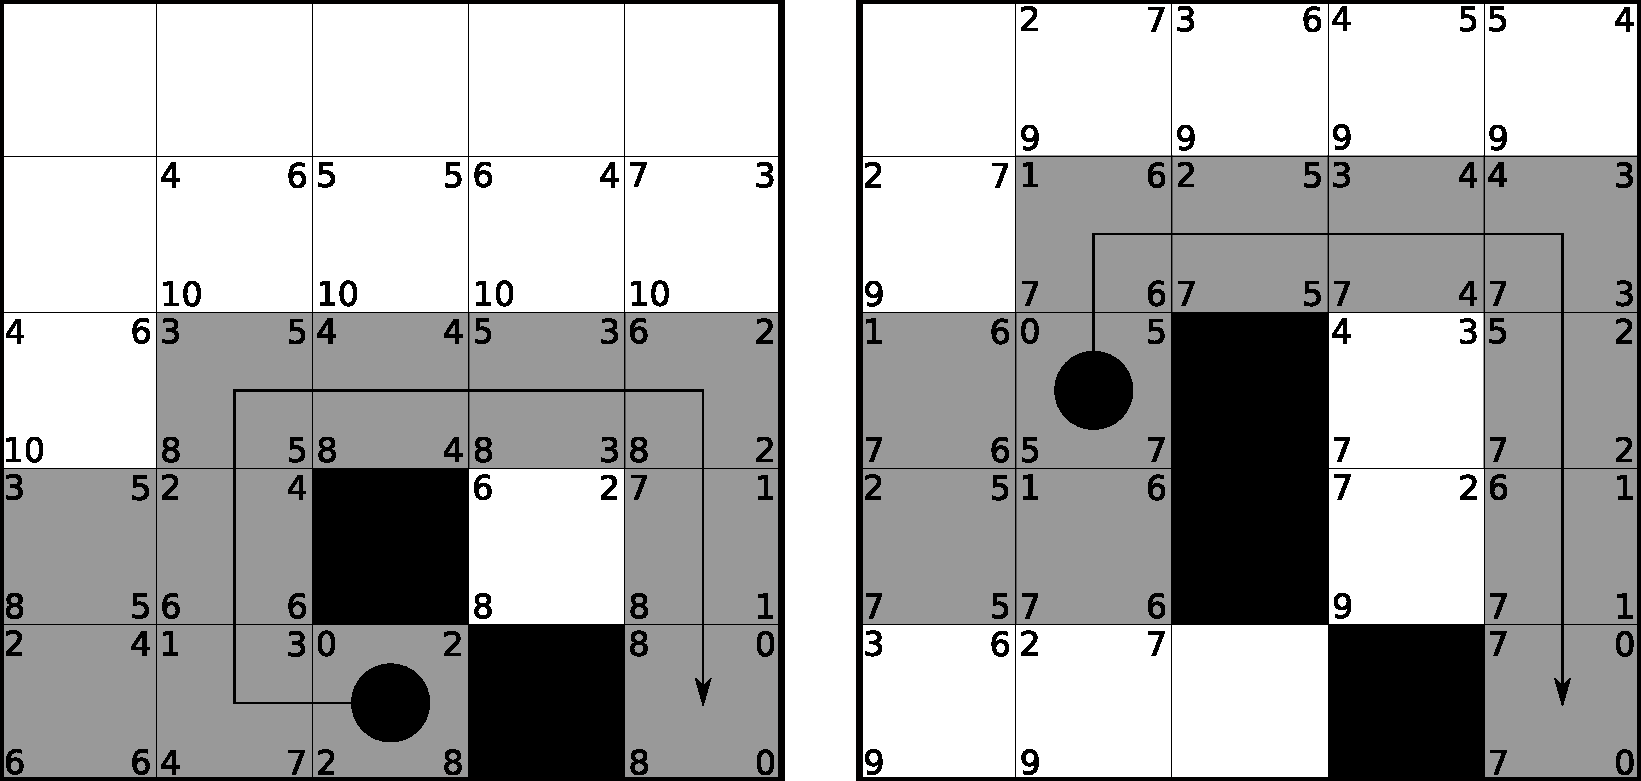
\includegraphics[width=0.9\linewidth]{images/rtaastar.pdf}
	\caption{Primjer pretrage RTAA*\cite{article:RTAAStar}}
	\label{fig:rtaastar}
\end{figure}

\par Na slici~\ref{fig:rtaastar} prikazan je primjer pretrage RTAA*.
Maksimalni broj pretraženih stanja u ovoj pretrazi nije ograničen, kao ni maksimalni broj poteza koje agent može napravit.
Kao i s primjerom na slici~\ref{fig:pathfindingCycle}, u gornjem lijevog kutu prikazan je trošak \(g(s)\), u gornjem desnom \(h(s)\), u donjem lijevom \(f(s)\) te siva polja označavaju pretražena stanja.
Heuristička funkcija je definirana kao zbroj horizontalne i vertikalne udaljenosti do cilja, što je poznatije pod nazivom ''Manhattan heuristika''.

Nakon prve pretrage, agent se pomaknuo do pozicije \((1, 2)\) kada se na  terenu uočena iznenadna promjena: na poziciju \((2, 2)\) dodana je prepreka.
Pošto se ta pozicija nalazi na putu do cilja, potrebno je ponoviti pretragu.
Prva pretraga ažururala je vrijednosti heuristika \(h(n)\) za sva pretražena stanja, što se vidi u donjem lijevom kutu ćelija.
U drugoj pretrazi, te se vrijednosti gledaju kao heurističke vrijednosti za njihova stanja, što sprijećava pretragu da se usmjeri prema prijašnjoj početnoj pozicij, odnosno \((2, 0)\).

\section{Grupiranje jedinica}\label{sec:grouping}

\par Algoritam A* i njegove varijacije su sposobne pronaći putanju do cilja ali ne uzimaju u obzir taktičko pozicioniranje jedinica. 
Primjerice, ako igrač u RTS igri odjednom odabere više od jedne jedinice i zada im odredište, očekivano ponašanje je da će se jedinice zajedno kretati kao skupina. 
Također, u borbi je poželjno se jedinice nastoje pozicionirati na maksimalnoj udaljenosti od mete na kojoj i dalje mogu pucati, kao što se može vidjeti na slici~\ref{fig:enemySeparation}.

\begin{figure}[h]
	\centering
	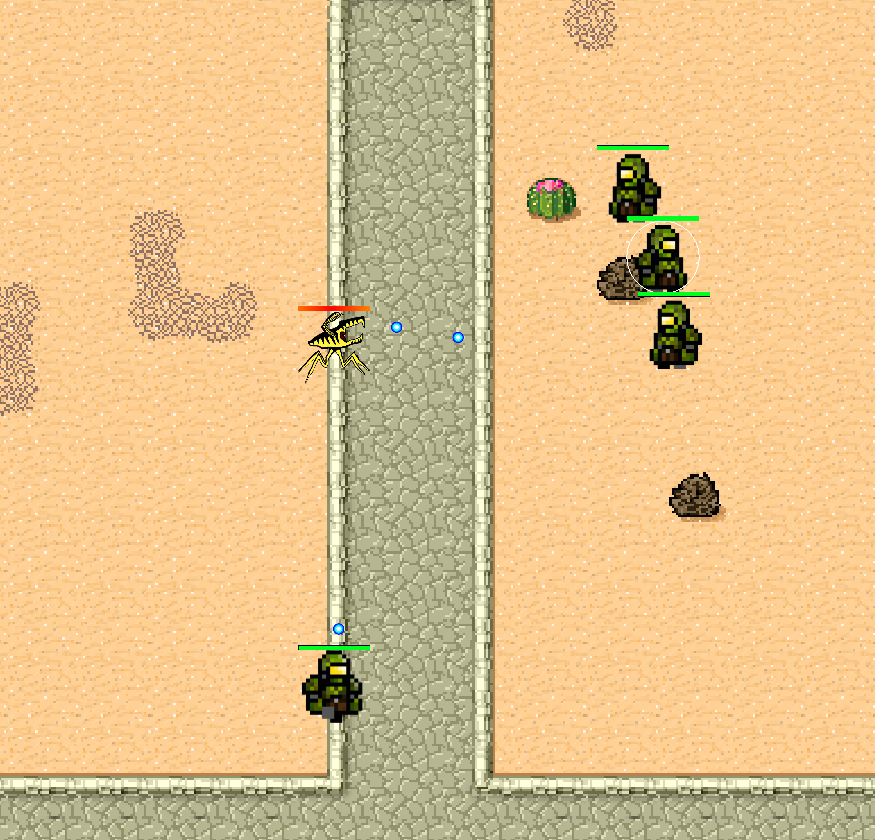
\includegraphics[width=0.5\linewidth]{images/enemySeparation.png}
	\caption{Pozicioniranje jedinica na maksimalnoj udaljenosti od mete}
	\label{fig:enemySeparation}
\end{figure}

% TODO this isn't finished

\subsection{Algoritam \textit{Boids}}\label{ssec:boids}

\par Kada se jedinice grupiraju, njihovo kretanje prema cilju mora biti zajedničko.
Kada bi prilikom zadavanja cilja grupi jedinica za svaku jedinicu pokrenuli algoritam A*, oni bi se kretali neovisni jedni o drugima. 
Zbog njihovih različitih pozicija, njihove putanje bi također mogle biti drastično različite. 
Također, ako se jedinice kreću po istim putanjama one će se često sudarati međusobno. 
Ovakav rezultat nije prihvatljiv s obzirom na očekivanje da će grupa jedinica biti jača i efikasnija od jedne same jedinice.

\par Inspiracija za implementaciju grupiranja jedinica dolazi iz prirode. 
Kretanje jata ptica ili plove riba je sinkronizirano i fluidno iako se sastoji od kretanja mnogih individualnih životinja, gdje se ponašanje svake od njih temelji samo na njenoj lokalnoj percepciji svijeta.
Algoritam koji primjenjuje osnovno ideje ponašanja jata ptica i primjenjuje ih na ostale probleme zove se \textit{Boids}, što dolazi iz engl. \textit{bird-like objects}, odnosno \textit{birdoids}\cite{article:FlocksHerdsSchools}.

\par Najosnovnija inačica algoritma \textit{Boids} sastoji se od tri pravila:
\begin{itemize}
	\item \textbf{odvojenost}: usmjeravanje jedinica kako bi se izbjegli sudari sa suborcima.
	\item \textbf{poravnatost}: usmjeravanje jedinica prema prosječnom smjeru kretanja grupe.
	\item \textbf{kohezija}: usmjeravanje jedinica prema centru mase grupe. 	 
\end{itemize}
Dodatna pravila se mogu dodati, poput zajedničkog kretanja prema trenutnom cilju, izbjegavanja sudara sa zgradama, izbjegavanje protivničkih jedinica, itd.

\par Algoritam \textit{Boids} ima razne ostale primjene, poput stabilizacije bespilotnih letjelica, izrade animacija te primjene u optimizacijskim problemima poput roja čestica (engl. \textit{Particle swarm optimization}).

\begin{figure}[h]
	\centering
	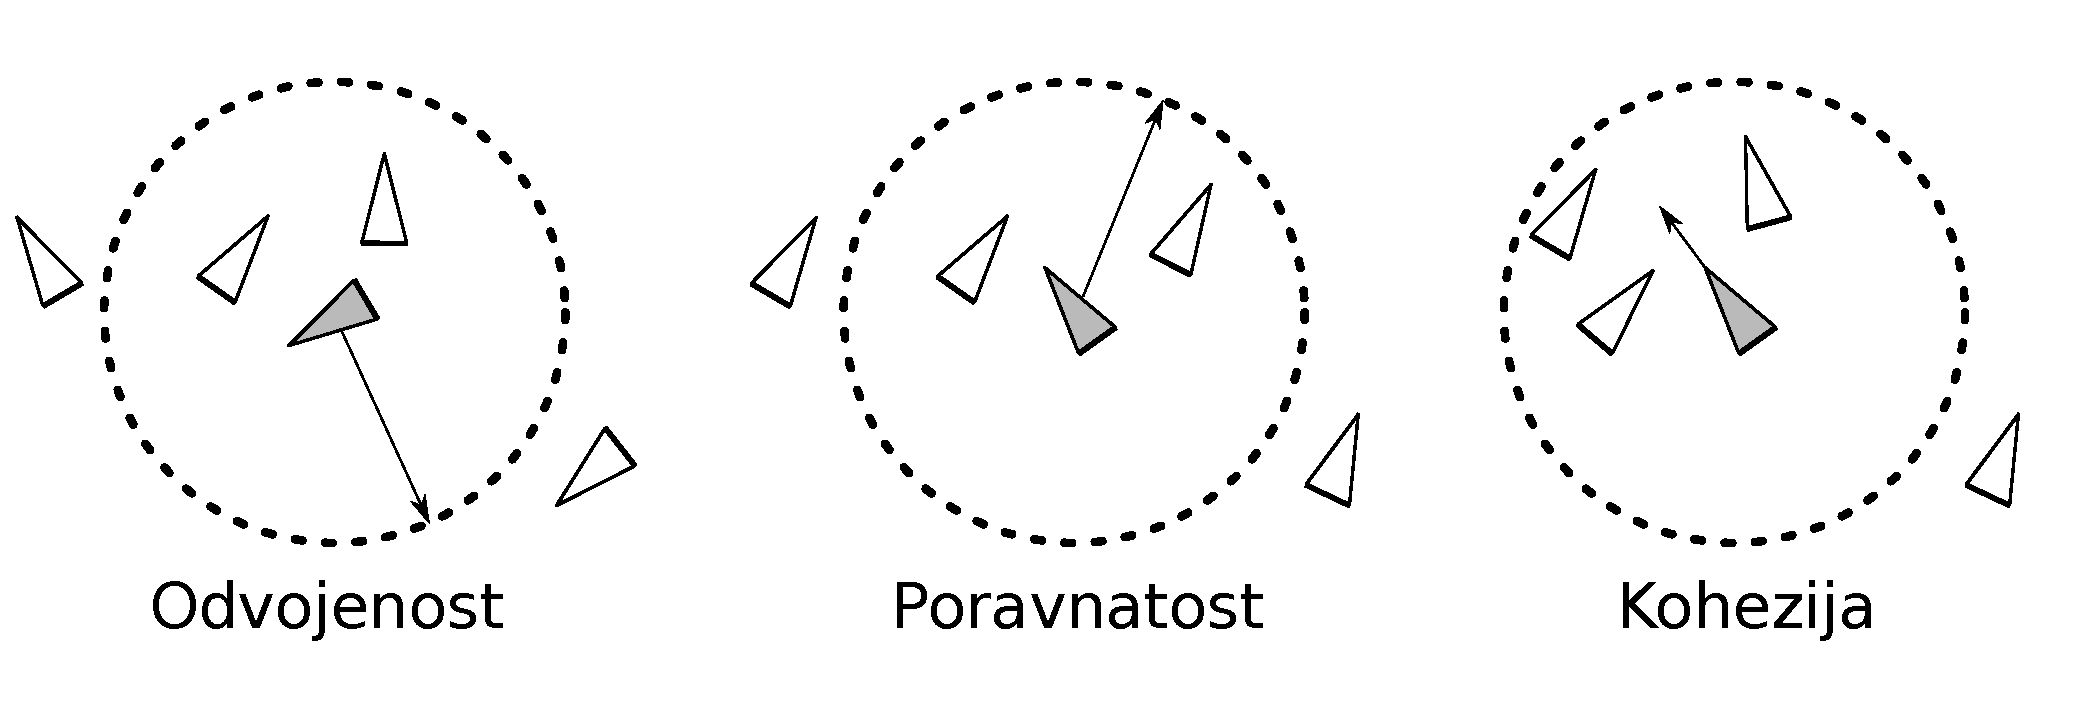
\includegraphics[width=1.0\linewidth]{images/boids.pdf}
	\caption{Tri osnovna pravila za algoritam \textit{Boids}}
	\label{fig:boids}
\end{figure}

\par Na slici~\ref{fig:boids} vizualizirana su navedena pravila odvojenosti, poravnatosti i kohezije. 
Sivi trokut predstavlja jedinicu nad kojom se navedene operacije trenutno obavljaju, dok iscrtani krug oko njega predstavlja radius u kojem promatra ostale jedinice. 
Na crtežu za odvojenost na trenutni trokut djeluju dva trokuta iznad njega, što mu mijenja smjer prema smjeru označenim sa strelicom. 
U crtežu za poravnatost vektor smjera usmjeruje se prema smjeru prema kojem ostale jedinice putuju. 
U zadnjem crtežu vidi se primjer kohezije, odnosno smjer trenutnog trokut se zakreće prema prosječnoj poziciji ostalih trokuta u radiusu.

\subsection{Hibridna navigacija}\label{ssec:hybrid}

\par Uz pomoć algoritma A* i algoritma \textit{Boids} postignuta je mogućnost kretanja skupine jedinica zajedno po mapi.
Sljedeća ideja je proširiti algoritam \textit{Boids} kako bi mogao rješavati problem taktičkog pozicioniranja jedinica u borbi.
Metoda navigacije u kojoj se jedinice kreću po mapi prema algoritmu A* dok nisu u blizini protivničkih jedinica i zgrada, a inače prevladava algoritam \textit{Boids}, naziva se hibridna navigacija (engl. \textit{hybrid pathfinding})\cite{article:HybridPathdinding}.

\par Algoritam \textit{Boids} bit će modificiran tako da nastoji držati jedinice na maksimalnoj udaljenosti od neprijateljskih jedinica i zgrada na kojoj i dalje mogu pucati.
To se postiže tako da se u pravila za algoritam \textit{Boids} doda uvjet kada se protivnička meta pojavi unutar radijusa napada jedinice, njen vektor smjera se mijenja u smjeru suprotnom od protivničke pozicije.
Ako je riječ o jedinici s ograničenim ili nepostojećim borbenim sposobnostima poput radnika, njen cilj je držati se na udaljenosti većoj od protivničkog radijusa za napad.
Ovo se pravila može proširiti i da vrijedi u slučaju da je borbena jedinica odlučno nadjačana, npr. ako jedna slaba jedinica naiđe na suparničku skupinu jačih jedinica.

\begin{figure}[h]
	\centering
	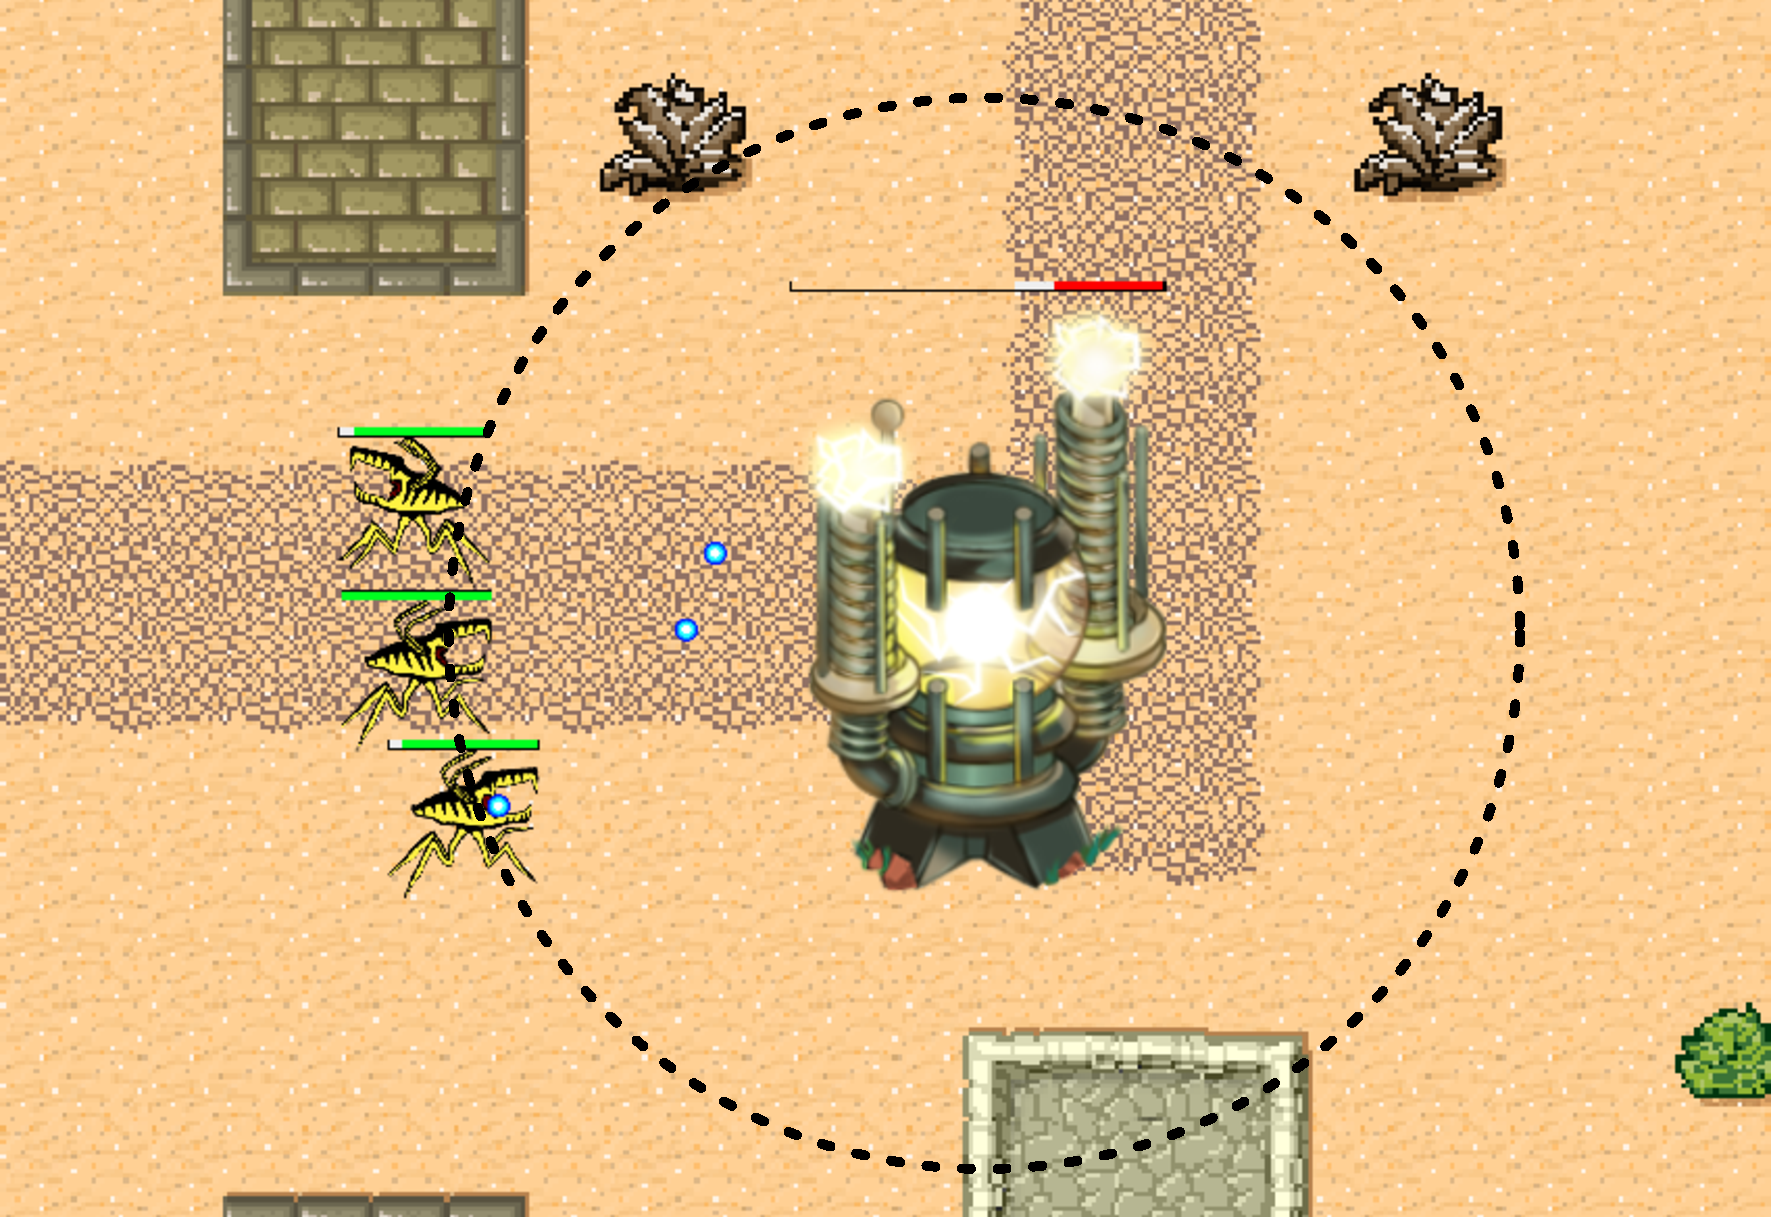
\includegraphics[width=0.8\linewidth]{images/boidsEnemySeparation.pdf}
	\caption{Odvajanje od protivničkih zgrada}
	\label{fig:boidsEnemySeparation}
\end{figure}

\par Na slici~\ref{fig:boidsEnemySeparation} prikazan je primjer u kojem su jedinice kojima upravlja bot\footnote{računalni program koji obavlja automatizirane poslove, poput upravljanja neprijateljskih jedinica protiv igrača} napale zgradu od ljudskog igrača.
Iscrtkanom kružnicom označena je maksimalna udaljenost s koje protivničke jedinice mogu pucati po igračevoj zgradi, te je vidljivo kako se protivničke jedinice drže te udaljenosti.

\chapter{Implementacija jezgrenih funkcionalnosti}\label{ch:implementation}

\par Programska implementacija napisana je u programskom jeziku Java, uz uporabu besplatne biblioteke otvorenog koda \textit{LibGDX}.
Biblioteka \textit{LibGDX} omogućava izradu mobilnih i \textit{desktop} igara koristeći istu bazu programskog koda. 
Za izradu i uređivanje mape korišten je besplatni uređivač mapa \textit{Tiled}.

\par Programska implementacija izdvojena je u tri glavna modula:
\begin{itemize}
	\item \textit{pathfinding}: sadrži generalizirane strukture podataka i algoritme pretrage.
	\item \textit{genericRTS}: sadrži generične funkcionalnosti RTS igre, poput jedinica, zgrada i podsustava za kretanje jedinica.
	\item \textit{core}: sadrži konkretan prototip RTS igre napisane koristeći prijašnja dva modula.
\end{itemize}

\section{Izdvajanje jezgrenih funkcionalnosti}

\subsection{Objekti u igri}

\par U paketu \textit{hr.fer.zemris.zavrsni.rts.objects} iz modula \textit{genericRTS} nalazi se apstraktni razred \textit{AbstractGameObject} koji predstavlja sve objekte u igri.
U njemu se nalaze informacije o poziciji objekta, njegovoj veličini, vektoru kretanja, itd.

\par Iz njega se izvode 4 podrazreda bitna za generičnu funkcionalnost RTS igre:
\begin{itemize}
	\item \textit{Building}: modelira zgradu koje se nalaze na mapi.
	\item \textit{Resource}: modelira izvor resursa na mapi.
	\item \textit{Projectile}: modelira projektil, poput metka, koji leti po mapi i vrši štetu nad metom koju pogodi.
	\item \textit{Unit}: modelira jedinicu, te pozivu logiku za samostalno kretanje jedinica. 
\end{itemize}
Također je prisutno sučelje \textit{ISquad} koji predstavlja grupu jedinica i njegove implementacije su zadužene za zajedničko kretanje jedinca.

\begin{figure}[h]
	\centering
	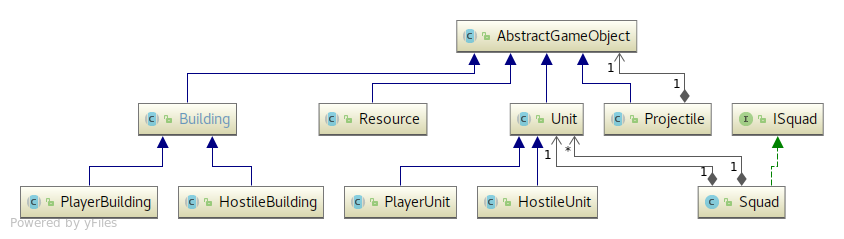
\includegraphics[width=0.8\linewidth]{images/umlObjects.png}
	\caption{Hijerarhija objekata u igri}
	\label{fig:umlObjects}
\end{figure}

\par Na slici~\ref{fig:umlObjects} vidljiva je opisana hijerarhija objekta.
Također su vidljivi tipovi \textit{PlayerUnit} i \textit{HostileUnit}, odnosno jedinice koje su na strani igrača i računala respektivno.
Isto to vrijedi i za tipove \textit{PlayerBuilding} i \textit{HostileBuilding}.
Dodatno, prikazan je tip \textit{Squad} koji implementira sučelje \textit{ISquad}.

\subsection{Uređivanje mape}

\par Alat za uređivanje mapa \textit{Tiled} nudi grafičko sučelje u kojem korisnik definira izgled terena i može pridijeliti dodatne podatke za lokacije, tipove terene ili mapu općenito.
Također nudi opciju izvoza izrađene mape u format \textit{TMX}\footnote{engl. \textit{Tiled map XML}}.
Uvoz i prikaz mapa u navedenom formatu je podržan unutar biblioteke \textit{LibGDX}.

\par Budući da je uređivanje mape implementirano uporabom alata \textit{Tiled} i formata \textit{TMX}, ovaj aspekt igre je većinom također neovisan o konkretnoj implementaciji.
Mapa se sama po sebi prikazuje kao niz pločica s teksturama na 2D plohi.
Taj dio dizajna mape može biti dijeljen između mnoštva igara iz različitih žanrova osim RTS-a.

\par Međutim, za bilo kakvu interakciju s mapom, potrebne su dodatne informacije.
Konkretno za RTS, kako bi jedinice pronašle najkraći put po mapi, igra mora pristupiti informaciji o tome gdje jedinica smije ili ne smije proći, na kojim mjestima se jedinica može kretati brže ili sporije, itd.
Primjerice, jedinica će se brže kretati po cesti nego po pijesku.
Jednostavni pristup za rješavanje tog problema je za svaku vrstu podloge na  terenu definirati modifikator brzine kretanja od 0 do 1.

\begin{figure}[h]
	\centering
	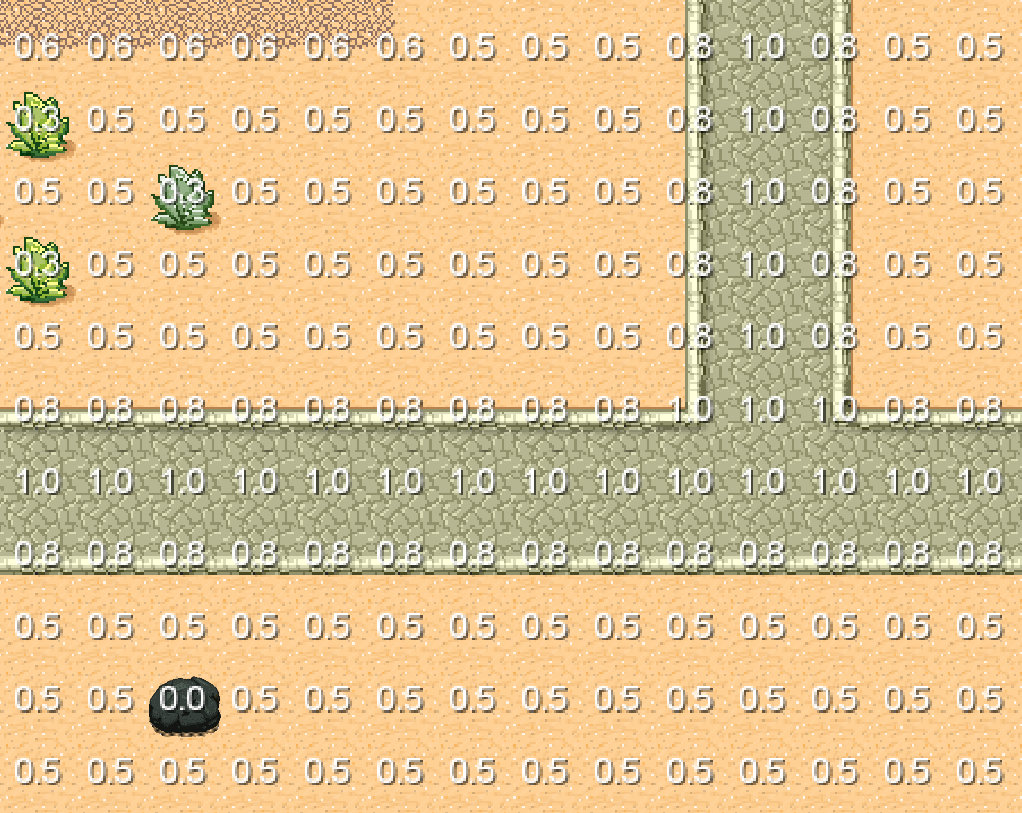
\includegraphics[width=0.6\linewidth]{images/tileModifiers.png}
	\caption{Prikaz modifikatora kretanja na mapi}
	\label{fig:tileModifiers}
\end{figure}

\par Na slici~\ref{fig:tileModifiers} prikazan je primjer gdje svaka pločica na mapi ima definiran modifikator brzine kretanja ovisno o svojem materijalu.
Žućkasta dio terena predstavlja pjesak, dok siva kamena tekstura predstavlja cestu.
Kao što se vidi, na cesti je modifikator kretanja \(1.0\) dok je na samom pjesku brzina kretanja dvostruko manje, odnosno \(0.0\).
Također, u gornjem lijevog kutu prikazani su grmovi kroz koje se jedinica može još sporije kretati, uz modifikator \(0.2\).

\par Konačno, zadnji skup podataka koji mora biti zapisan u opisu mape su položaji konkretnih resursa, zgrada i jedinica.
% TODO nastaviti o ovome, napisati kako je to ovisno o konkretnoj igri i opisati kako je rijeseno u ovoj igri

\subsection{Kretanje jedinica}

\par U modulu \textit{pathfinding} nalaze se strukture podataka za izvršenje pretrage prostora stanja.
Primjerice, sučelje \textit{ISearchProblem} definira problem pretrage, odnosno početno stanje, provjeru krajnjeg stana i izračun idućih stanja i akcija. 
Također su definirana sučelja \textit{IHeuristic} koji definira funkciju heuristike i \text{ISearchAlgorithm} koji definira algoritam pretrage nad problemom s definiranom heuristikom.

% TODO

\section{Konkretna implementacija}

\par Uz opisanu jezgrenu funkcionalnost RTS igre, izrađen je prototip jedne konkretne igre koja sadrži opisane osnovne funkcionalnosti.
U navedenoj igri igrač započne igru s bazom i jednim robotskim radnikom.
Baza je okružena s mineralima koje radnik može skupljati.
Sa skupljenim mineralima moguće je izgraditi nove radnike, vojnike i defenzivnu građevinu koja će pucati na neprijatelje.

\par Jedinice se u igri odabiru tako da igrač povuće lijevi klik miša, što se vizualizira pravokutnikom koji predstavlja označeno područje, čime se označavaju sve jedinice unutar tog pravokutnika.
Igrač zatim zadaje naredbe jedinicama koje su trenutno označene tako da klikne na proizvoljnu poziciju na mapi s desnim klikom miša.
Označene jedinice će se zatim grupirati ako su dovoljno blizu i krenuti zajedno prema cilju.

\begin{figure}[h]
	\centering
	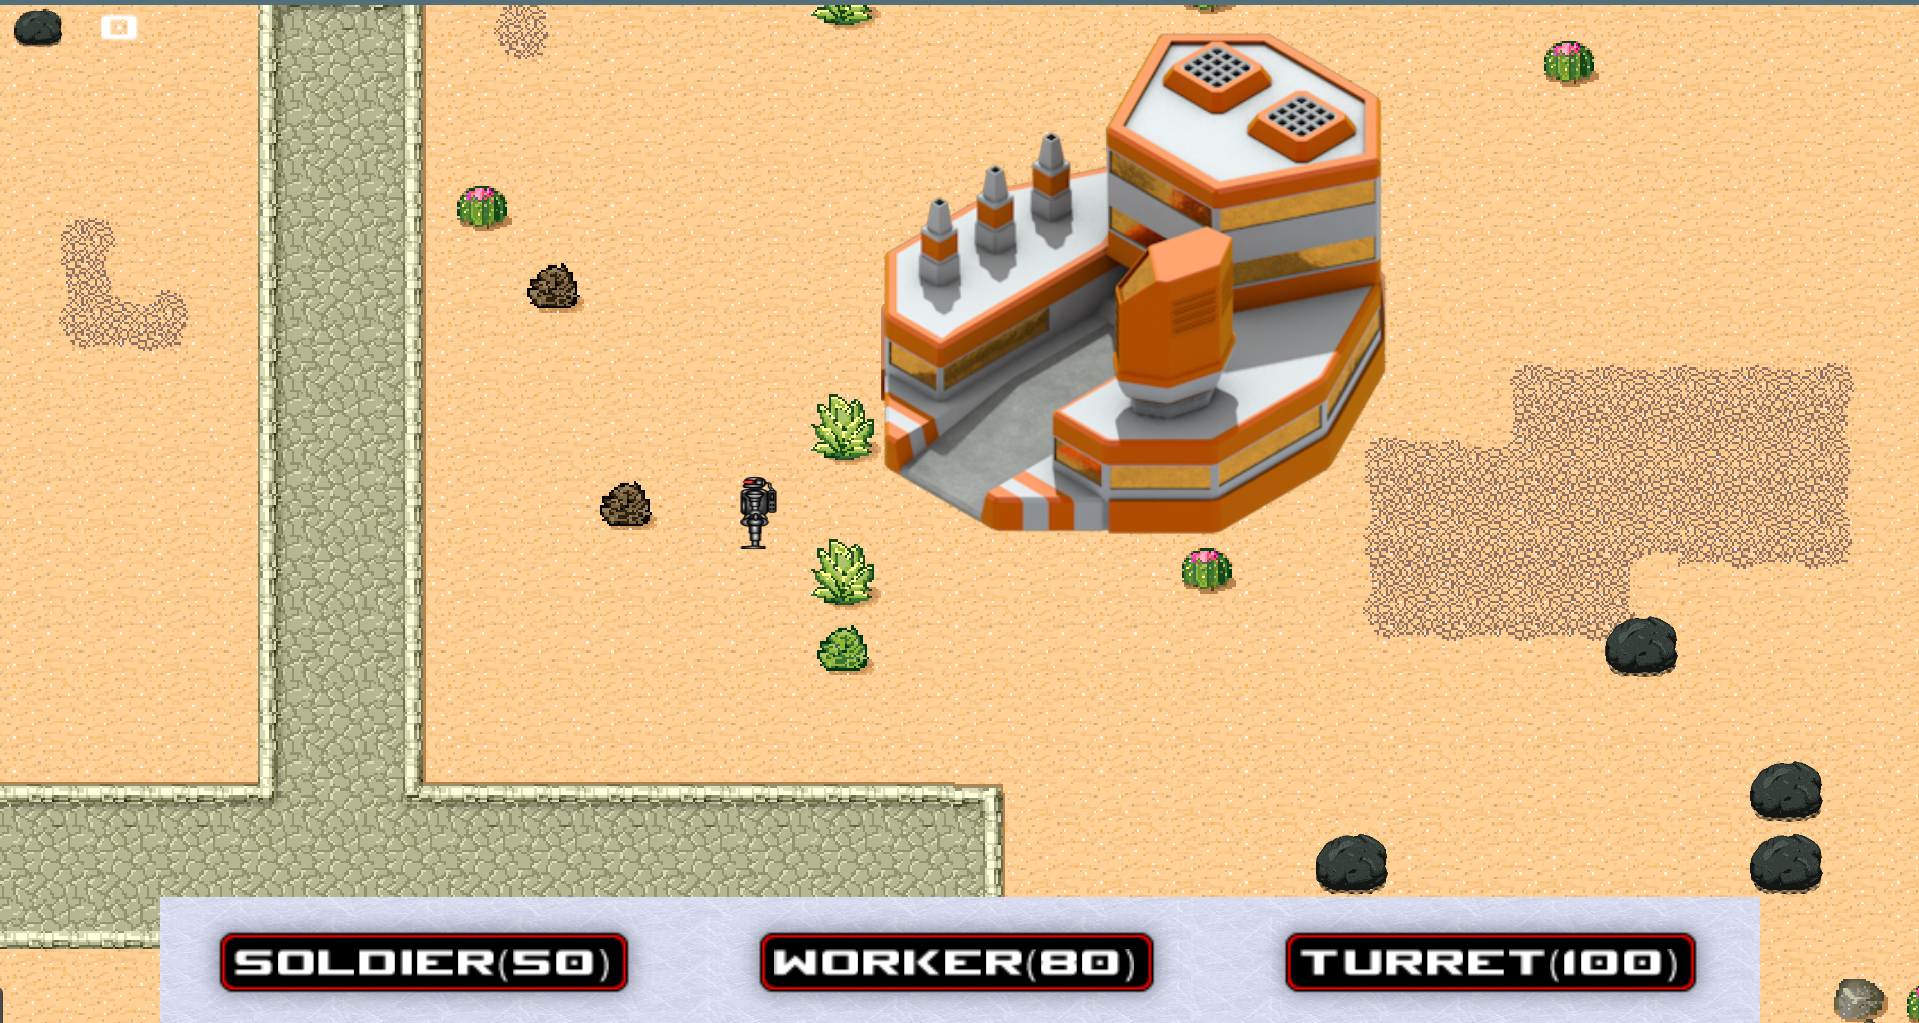
\includegraphics[width=0.9\linewidth]{images/gameStartScreenshot.png}
	\caption{Početno stanje u igri}
	\label{fig:gameStart}
\end{figure}

\par Na slici~\ref{fig:gameStart} prikazano je početno stanje pri pokretanju nove igre.
Narančasta zgrada predstavlja igračevu bazu, te se lijevo od nje nalazi robotski radnik.
Crne stijene desno ispod baze predstavljaju izvore minerala.
Ikona minerala u gornjem lijevom kutu s brojkom 0 pored nje predstavlja količinu skupljenih minerala koji dosad nisu potrošeni.
Na dnu ekrana se također nalazi izbornik iz kojeg igrač bira na što želi trošiti resurse, te je u zagradama napisana cijena prikazanog izbora, te crveni obrub oko tipke označava nemogućnost odabira zbog manjka resursa.

\par Na učitanoj mapi također su prisutne neprijateljske baze.
One će otprilike svakih 10 sekundi stvoriti neprijateljsku jedinicu.
Kada jedna neprijateljska baza stvori 3 jedinice, one se grupiraju i krenu u napad prema igračevoj bazi.
Da bi se stigao pripremiti, igrač se mora čim prije moć obraniti te nakon toga krenuti u napad.
Cilj u igri je uništiti sve neprijateljske jedinice i baze na mapi, bez da igrač izgubi vlastitu bazu. 

\begin{figure}[h]
	\centering
	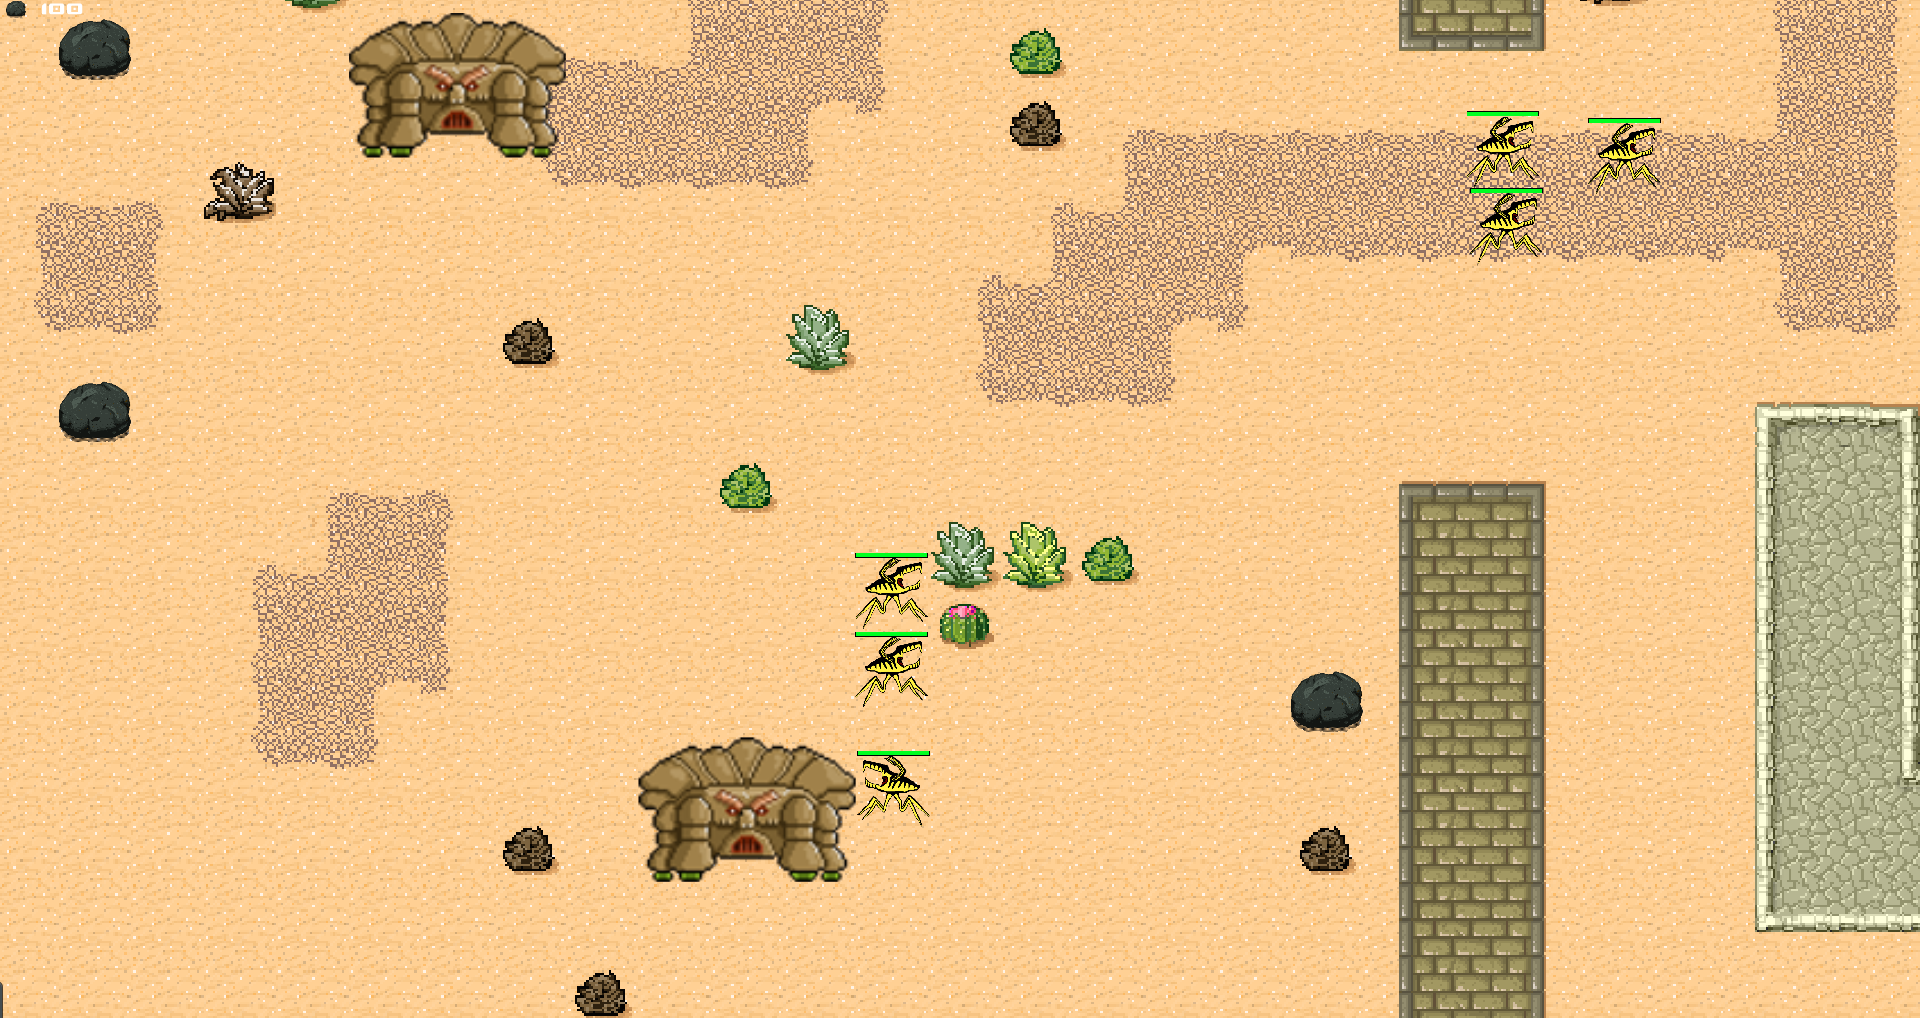
\includegraphics[width=0.9\linewidth]{images/enemyBases.png}
	\caption{Neprijateljske baze u igri}
	\label{fig:enemyBases}
\end{figure}

\par Na slici~\ref{fig:enemyBases} prikazane su neprijateljske baze i dvije skupine od tri jedinica koje kreću u napad na igračevu bazu.

\par Borba započinje kada se igračeva jedinica nađe u dometu protivničke jedinice, ili suprotno.
Čim se dvije jedinice s različitih strana nađu u blizi, one počnu pucati jedna na drugu.
Protivničke jedinice koriste hibridnu navigaciju opisanu u potpoglavlju~\ref{ssec:hybrid}, odnosno nastoje se držati na maksimalnoj udaljenosti od igračevih jedinica na kojoj mogu i dalje pucati, najčešće formirajući polukrug oko navedene mete.

\begin{figure}[h]
	\centering
	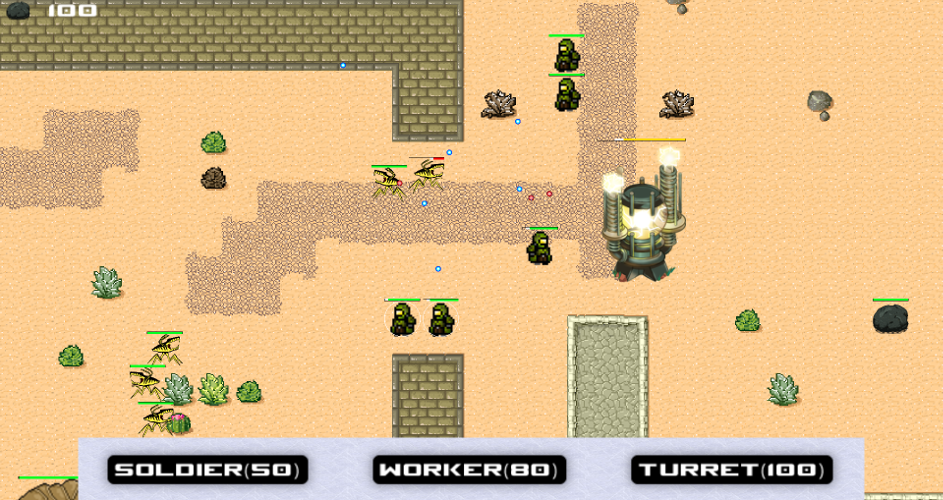
\includegraphics[width=0.9\linewidth]{images/battle.png}
	\caption{Prikaz borbe u igri}
	\label{fig:battle}
\end{figure}

\par Na slici~\ref{fig:battle} prikazan je primjer borbe u igri.
Pet igračevih vojnika bore se protiv dviju protivničkih jedinica te im u bitci pomaže defenzivni toranj koji također puca na protivnike.
Iz lijevog donjeg kuta se približava idući val neprijateljskih jedinica.
Iznad svake jedinice i zgrade nalazi se crta koja označava njihovo trenutno ''zdravlje''.
Puna zelena crta označava da jedinica ili zgrada nije ozlijeđena, dok crvena skoro prazna crta znači da je jedinica pred smrti.
Također je vidljivo da igračeve jedinice pucaju plave metke, dok protivničke jedinice pucaju crvene.

\par Resursi u igri se skupljaju tako da igrač odabere radnika i naredi mu da se skuplja određeni izvor resursa, odnosno izvor minerala.
Naredba za skupljanje se zadaje tako da se stijena klikne s desnim klikom miša s izabranim radnikom.
Radnik će zatim pronaći put do navedenog resursa i početi ga skupljati kada mu dođe u blizinu.
Nakon što se resurs skupi, odgovarajuća količina minerala bit će dodana igraču.
Također, ako u blizini postoje ostali izvori materijala, radnik će ih samoinicijativno krenuti skupljati.
Bez ove mogućnosti, radnici bi zahtijevali previše mikroupravljanja te bi igrač redovito morao skretati pozornost s bitke samo kako bi zadao jednostavnu naredbu radniku.

\par Kada je skupljeno dovoljno minerala za izgraditi zgradu, igrač može klikom na gumb \textit{Turret (100)} izabrati da želi izgraditi navedenu zgradu.
Time će se pojaviti silueta zgrade koja prati lokaciju koju miš označuje na mapi, kao što je prikazano na slici~\ref{fig:building}.
Korisnikovim klikom na lokaciju na mapi će zgrada biti izgrađena na tom mjestu, ako je moguće.
Ako korisnik označi lokaciju na kojoj se zgrada ne može izgraditi, ili ako za izgradnju zgrade nisu dostupni resursi, silueta zgrade će biti crvena.

\begin{figure}[h]
	\centering
	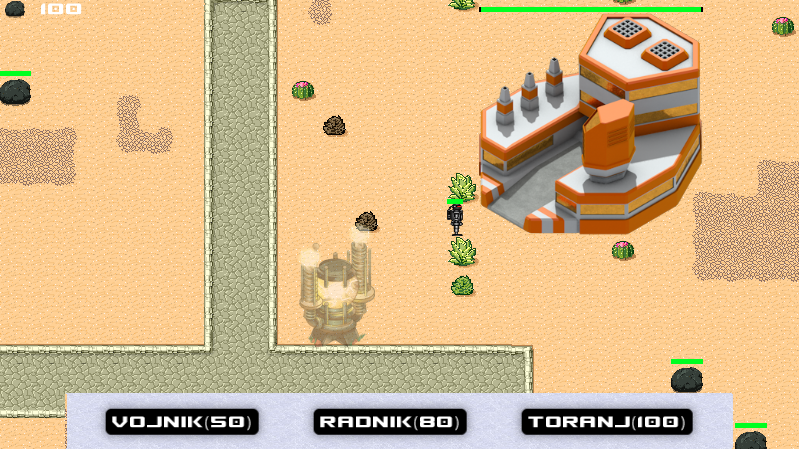
\includegraphics[width=0.9\linewidth]{images/building.png}
	\caption{Izgradnja novih zgrada u igri}
	\label{fig:building}
\end{figure}

\par Prilikom ulaska u igru igrač ima mogućnost pokretanja nove igre, učitavanja već započete igre, ulaska u postavke i izlazka iz igre.
% Dodaj slike
% Pokaži postavke

\section{Dodavanje novih funkcionalnosti}

Jedna od ključnih ideja tijekom razvoja jezgrenih funkcionalnosti RTS igre bila je jednostavno proširivost igre.
U ovom potpoglavlju biti će prikazano nekoliko primjera kako se mogu jednostavno dodati nove zgrade i jedinice u konkretnu igru.

\begin{minipage}{\textwidth}
	\lstinputlisting[caption = {Isječak koda u Javi koji dodaje novu protivničku jedinicu},
    label={fig:codeStickman}]{codesnippets/stickman.java}
\end{minipage}\

\par U programskom isječku~\ref{fig:codeStickman} prikazan je programski isječak za dodavanje nove jedinice.
Tekstura kojom će se jedinica prikazivati spremljena već je izrađena i učitana u jedinstvenom objektu \textit{Assets}, kojem se pristupa iz metode \textit{loadAnimation()}.
Tijekom nasljeđivanja razreda \textit{HostileUnit}, potrebno je definirati sve atribute koji mogu biti različiti za svaku jedinicu.
Ova konkretna jedinica ima natprosječnu brzinu kretanja i brzinu napada, no ima nisko zdravlje i moć napada.

\par Implementacija je također implementirala sučelje \textit{IBuildableUnit}, što definira metodu \textit{getTrainingCost}.
Ovo daje informaciju igri o utrošku rada koji je potreban da se jedinica ovog tipa izgradi.
Primjer tog rada je kada igrač da naredbu da se izgradi vojnik, igračeva baza će obaviti količinu rada koja je definirana u navedenoj metodi za vojnika.

\par Uz pretpostavku da tekstura za ovu jedinicu uspješno napravljena, navedeni isječak koda je dovoljan da ona bude funkcionalna unutar igre.
Nažalost, s obzirom na činjenicu da je u prijašnjem isječka dodana samo definicija jednice, ostatak igre ne zna za nju zbog čega se ona ne može prirodno pojaviti u igri.

\par Taj problem će se riješiti dodavanjem novog tipa zgrade.
Sve što treba napraviti je nasljediti razred \textit{HostileBuilding} i implementirati logiku s kojom će ta zgrada stvarati primjerke jedinica \textit{Stickman}, kao što je prikazano u programskom isječku~\ref{fig:codeStickmanSpawner}.
 
\begin{minipage}{\textwidth}
	\lstinputlisting[caption = {Isječak koda u Javi koji dodaje novu zgadu},
    label={fig:codeStickmanSpawner}]{codesnippets/stickmanSpawner.java}
\end{minipage}

\par U navedenom isječku nadjačana je metoda \textit{update} koja se pozove u svakoj iteracij igrine glavne petlje.
U svakom pozivu metode \textit{update} obavlja se određeni rad prema stvaranju nove jedinice, koja se zatim dodaje u igru pozivom metode \textit{spawnUnit}.

\par Sada je nova zgrada spremna da bude funkcionalna unutar igre tako što može stvarati primjerke jedinica tipa \textit{Stickman}, što je viljivo na slici~\ref{fig:stickman}.

\begin{figure}[h]
	\centering
	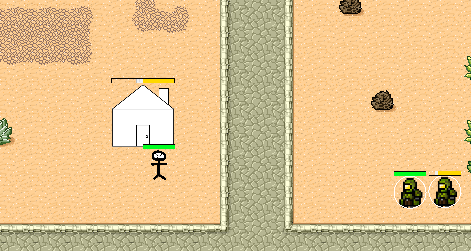
\includegraphics[width=0.7\linewidth]{images/stickman.png}
	\caption{Implementacija dodatnih funckionalnosti u igri}
	\label{fig:stickman}
\end{figure}

\par Definirani postupak dodavanja osigurava da nove zgrade i jedinice nisu ovisne o konkretnoj implementaciji ijedne RTS igre.
Bilo koja RTS igra koja koristi opisani podsustav može slobodno koristiti objekte \text{Stickman} i \textit{StickmanSpawner}.

\par Isti taj postupak je analogan i za dodavanje novih izvora resursa.
Komplikacija sa dodavanjem novih izvora resursa nastaje zato jer moraju definirati koji će resurs dodati igraču kada se unište.
U ovom podsustavu, resurs prilikom uništenja pošalje igri odgovarajuću količinu resursa i ključ koji ga definira.
Zahvaljujući tome, bilo koja konkretna implementacija RTS igre koja koristi minerale kao resurs može koristiti bilo koje izvore minerala, dokle god je dogovoreni isti ključ.
U prikazanoj konkretnoj implementaciji minerali su označeni ključem \textit{minerals}.

\chapter{Zaključak}\label{ch:conclusion}
Zaključak.

\bibliography{literatura}
\bibliographystyle{fer}

\begin{sazetak}
Računalne igre jedan su od vrlo značajnih pokretača razvoja računala. Postoji mnoštvo vrsta računalnih igara. 
Jednu od vrlo interesantnih vrsta igara čine strategije u stvarnom vremenu (engl. Real-Time Strategy, RTS). 
Razvoj takvih igara općenito uključuje pisanje mnogih podsustava i razvoj funkcionalnosti koje nisu specifične za konkretnu igru već ih je moguće višestruko iskorištavati. 
Takve funkcionalnosti moguće je izolirati u zaseban razvojni okvir. U okviru završnog rada potrebno je proučiti koji su sve elementi prisutni u RTS igri. 
Potrebno je napraviti programsku implementaciju osnovnih podsustava koje će biti moguće dijeliti između različitih RTS-igara. 
Također je potrebno implementirati prototip jedne konkretne igre koja sadrži osnovne elemente poput prikaza mape svijeta, stvaranja građevina različitih funkcija (proizvodnja, obrana) te jedinica, upravljanje jedinicama (grupiranje, zadavanje ciljeva: dolazak na zadani položaj, pucanje, prikupljanje resursa) i osnovno upravljanje protivničkim jedinicama. 
Implementaciju je potrebno ostvariti u programskom jeziku Java. 
Radu je potrebno priložiti algoritme, izvorne kodove i rezultate uz potrebna objašnjenja i dokumentaciju. 
Citirati korištenu literaturu i navesti dobivenu pomoć.

\kljucnerijeci{Ključne riječi, odvojene zarezima.}
\end{sazetak}

\engtitle{Implementation of RTS game core}
\begin{abstract}
Computer games are a significant catalyst in the development of computers. 
There are many genres of computer games. 
Real-Time Strategy games represent one of the more interesting genres. 
The development of those types of games is based on developing a variety of subsystems and functionalities which aren't specific for one game, and are thus fit for reuse. 
These functionalities can be isolated into a separate workspace. 
As part of thesis, it is necessary to study which elements are present in an RTS game and develop a program implementation of the basic subsystems which can be shared between various RTS games. 
A further requirement is to develop a game prototype which contains the basic elements, such as the construction of buildings with various functions (manufactory, defense) and units, the management of units (grouping, assigning a goal: arrival at a destination, shooting, resource gathering) and basic enemy control.
The implementation is to be written in the Java programming language. 
The completed assignment must be handed over along with the used algorithms, source code and results with the necessary explanations and documentation. 
The literature that was used must be cited along with the received help.

\keywords{Keywords.}
\end{abstract}

\end{document}